
% -------------------------------------------------------------------------------
% Preamble
% -------------------------------------------------------------------------------
\documentclass[a4paper, 11pt, twoside, openright, english]{memoir}
\usepackage{mypreamble}
\usepackage[a4paper,pdftex,margin=0.5in]{geometry}										% A4paper margins

%\setlength{\oddsidemargin}{2mm}												% Remove 'twosided' indentation
%\setlength{\evensidemargin}{2mm}



% ------------------------------------------------------------------------------
% Definitions (do not change this)
% ------------------------------------------------------------------------------
\newcommand{\HRule}[1]{\rule{\linewidth}{#1}} 	% Horizontal rule

\makeatletter							% Title
\def\printtitle{%						
    {\centering \@title\par}}
\makeatother									

\makeatletter							% Author
\def\printauthor{%					
    {\centering \large \@author}}				
\makeatother							


\usepackage{makeidx} %If you want to generate an index, automatically 

\usepackage{graphicx} %If you want to include postscript graphics 
\graphicspath{{./images/}}
\usepackage{zi4}
\def\ttdefault{inconsolata}

\usepackage[utf8]{inputenc}
\numberwithin{equation}{section}

\usepackage{listings}
\usepackage{xcolor}
\usepackage[toc]{glossaries}
%%%%%%%%%%%%%%%%%%%%%%%%%%%%%%%%%%%%%%%%%%%%%%%%%%%%%%
\lstdefinestyle{numbers} {numbers=left, stepnumber=1, numberstyle=\tiny, numbersep=10pt}
\lstdefinestyle{MyFrame}{backgroundcolor=\color{lightgray},frame=shadowbox}
\lstdefinestyle{MyCStyle} {language=C, style=MyFrame,frame=lines , basicstyle=\footnotesize\ttfamily}
\lstdefinestyle{MyJavaStyle} {language=Java,style=numbers,style=MyFrame,frame=lines , basicstyle=\footnotesize\ttfamily}
\lstdefinestyle{MyPythonStyle} {language=Python,style=numbers,style=MyFrame,frame=lines , basicstyle=\footnotesize\ttfamily}
% Set nJexl Language Style
\definecolor{darkgreen}{RGB}{0,102,0}
\definecolor{darkblue}{RGB}{0,0,102}
\definecolor{darkred}{RGB}{102,0,0}
\definecolor{darkgray}{RGB}{96,96,96}

\usepackage[T1]{fontenc}
\lstdefinestyle{JexlStyle}{
  language=jxl,
  basicstyle=\fontfamily{pcr}\bfseries\selectfont\color{darkblue}, % Global Code Style : Inconsolata
  commentstyle=\itshape\color{darkgray}, % style of comments
  keywordstyle=\color{darkred}, % style of keywords
  stringstyle=\color{darkgreen}, % style of strings
  extendedchars=true, % Allows 256 instead of 128 ASCII characters
  tabsize=2, % number of spaces indented when discovering a tab 
  showstringspaces=false, % lets spaces in strings appear as real spaces
  breaklines=true, % wrap lines if they don't fit
  frame=trbl, % draw a frame at the top, right, left and bottom of the listing
  frameround=tttt, % make the frame round at all four corners
  framesep=4pt % quarter circle size of the round corners
}
% Fix the red color for TOC  
\usepackage{hyperref} 
\hypersetup{%
  colorlinks = true,
  linkcolor  = black
}

\makeglossaries
\makeindex
%\includeonly{chaptr2} %If you just want to process chaptr2.tex 


\begin{document} 

% SVN info for this file
\svnidlong
{$HeadURL$}
{$LastChangedDate$}
{$LastChangedRevision$}
{$LastChangedBy$}

% Remove header and footer
\thispagestyle{titlepage}

\begin{center}
  \newlength{\parSepLength}
  \setlength{\parSepLength}{10ex}

  \Large
  \centering

  % Main title
  \thinRule\par
  \par\vspace{0.15\parSepLength}
  \begin{minipage}{\textwidth}
    \centering
    \fontsize{36pt}{20pt}\selectfont\titleColor\scshape
    The \\ nJexl \\ Programming Language  
  \end{minipage}
  \par\vspace{0.25\parSepLength}
  \par\thinRule

  \vspace{0.125\parSepLength}

  \begin{minipage}{\textwidth}
    \centering
    An Exetnsible and Embeddable JVM Language \\ for Business Development \\ and Software Testing \\
    Version 0.3+
  \end{minipage}

  \vfill

  % Author
  \begin{minipage}{\textwidth}
    \centering
    \Large
    Nabarun Mondal
  \end{minipage}

  \vfill

  % Logo and other info
  \begin{minipage}{0.8\textwidth}
    \centering
    \small
  \end{minipage}
\end{center}


\frontmatter 
\tableofcontents 
\chapter{Preface}
 
{\LARGE n}Jexl initially was a continuation of \href{http://commons.apache.org/proper/commons-jexl}{Apache Jexl}\index{apache jexl} project.
That project was not active for 17 months, and I needed to use it, so I forked it. The reason are to be found below.

\begin{subsection}{A brief History}

All I wanted is a language where I can write my test automation freely - i.e. using theories from testing.
The standard book, and there is only one for formal software testing is 
that of \href{http://www.amazon.com/Software-Testing-Techniques-2nd-Edition/dp/1850328803}{Beizer}.\index{Beizer}

There was no language available which lets me intermingle with Java POJOs and let me write my test automation (validation and verifications). 
Worse still - one can not write test automation freely using Java. 
As almost all of modern enterprise application are written using Java, it is impossible to avoid Java 
and write test automation : in many cases you would need to call appropriate Java methods to automate APIs.

Thus, one really needs a JVM scripting language that can freely call and act on POJOs.
The idea of extending JEXL thus came into my mind : a language that has all the good stuffs from
the vast Java libraries, but clearly not verbose enough.

After cloning JEXL - and modifying it real heavy - a public release in a public repository
seemed a better approach. There, multiple people can look into it, rather than one lone ranger working from his den.
And hence nJexl was born. The \emph{n} stands for \emph{Neo,New}, 
not \href{https://nmandalh.wordpress.com}{Noga}, which is, by the way, my nick name.

\end{subsection}

\begin{subsection}{An Open Challenge From Java Land}

This actually was an \href{http://steve-yegge.blogspot.in/2006/03/execution-in-kingdom-of-nouns.html}{open challenge}:


\emph{A noted PhD from Sun, read this essay, and had this to say: 
``hmm, chuckle :) This guy has too much time on his hands ! he should be doing useful work, or inventing a new language to solve the problems. Its easy to throw stones - harder to actually roll up your sleeves and fix an issue or two, or write/create a whole new language, and then he should be prepared to take the same criticism from his peers the way he's dishing it out for others. Shame - I thought developers were constructive guys and girls looking to make the lives of future software guys and girls easier and more productive, not self enamouring pseudo-intellectual debaters, as an old manager of mine used to say in banking IT - 'do some work' !''}


And I like to think that I just did. That too, while at home, in vacation time, and in night time 
( from 8 PM to 3 AM. - see the \href{https://github.com/nmondal/njexl/commits/master}{check-ins}.)
Alone. But the users are the best judge.

\end{subsection}


\begin{subsection}{About The Language}

It is an interpreted language. It is asymptotically as fast as Python \index{python}, with a general lag of 200 ms of reading and parsing files, where native python is faster. After that the speed is the same.
 
It is a multi-paradigm language. It supports functionals ( i.e. anonymous functions ) out of the box, and every function by design can take functional as input. There are tons of in built methods which uses functional.

It supports OOP. Albeit not recommended, as \href{http://harmful.cat-v.org/software/OO_programming/why_oo_sucks}{OOPs!} tells you.
clearly shows why. In case you want C++ i.e.  \href{http://en.wikipedia.org/wiki/Multiple_inheritance}{multiple inheritance} with full operator overloading, friend functions, etc. then this is for you anyways. 
Probably you would love it to the core.

Python is a brilliant language, and I shamelessly copied many, and many adages of Python here. The heavy use of  \_\_xxx\_\_    
literals, and the \emph{me} directive, and \emph{def} is out and out python. 

The space and tab debate is very religious, and hence JEXL is "{ blocked }" : Brace yourself.
Pick tab/space to indent - none bothers here.
You can use ";" to separate statements in a line. 
Lines are statements.

\end{subsection}


\begin{subsection}{Thanks}
And finally, all of these pages were typed using my trust worthy Mac Book Pro, at home using \href{http://pages.uoregon.edu/koch/texshop}{TexShop-64}.
So, thanks to Richard Koch, Max Horn Dirk Olmes. For \href{http://tug.org/mactex/}{MacTex}, thanks MacTex. You guys are great!
Thanks to Apple for creating such a beautiful systems to work on. Steve, I love you. RIP.
For Windows, the trusty \href{http://www.tug.org/texworks}{TexWorks} was used using \href{http://miktex.org}{MikeTex} packages. Thanks to you too!
In the end many a thanks to Gabriel Hjort Blindell - for the beautiful style file he created which can be found \href{http://web.ict.kth.se/~ghb/publications/documents/thesis-template.tar.gz}{here}. Gabriel, thanks a ton.
\end{subsection} 

\mainmatter 
\chapter{On Software and Business Development}\label{intro}

{\LARGE S}oftware is needed to do most of the business, and it is software development, that becomes sometime the bottleneck 
of the business development. Here, we discuss the goal of nJexl, the very problems it seeks to eradicate.


\begin{section}{Business Development}\label{buisness-development-defined}

Does business need software? No and Yes. \index{Hello Curry}
Clearly how brilliantly the code was written does not matter when one owns a portal like \href{www.hellocurry.com}{hello curry}.
Software augments business, there is no point making software the business. There are many firms doing software as business, and it is a very high niche game. In reality, most of the businesses are not about software, it is about taking user pain away, and alway - making end users happy. 

\emph{Marketing brings you customers, Tech-folks retain them. -- Anon}


\begin{subsection}{Needs of the Business}\label{business-need}\index{business needs}

Start with hello curry, whose game is to distribute food to the client. Hence it has a database full of food items, which it would showcase in the portal. User would click whatever she wants to eat, and checks out. The items gets delivered in time. Users can see their orders in a page. Occasionally, some specific food items gets added as the discounted price. Together, these requirements is what drives business for hello curry.

\end{subsection}

\begin{subsection}{Imperative Implementation}\label{imperative-impl}
\index{Imperative}

Certain things in the implementations are invariant,  one needs a database to store the users and their settings, and the food items. The code to showcase what to display as items are also fixed in nature. The real business problem is the \emph{discounted} one . Under normal circumstances, one would write this code :

\begin{lstlisting}[style=JexlStyle][float]
for ( item : items ){
   if ( discounted(item) ){
      display_item_discounted(item)
   }else{
     display_item(item)
   }
}
\end{lstlisting}

This sophomore level code is indeed correct when looked at in a very naive way.
But the whole new complexity of the business starts with this, and is a one way ticket to the land of more and more complexity and unmanageable code. To showcase, observe now, how one would have added 2 different discounted category? Of course, one needs to add \emph{necessary} code to the snippet :

\begin{lstlisting}[style=JexlStyle]
for ( item : items ){
   if ( discounted_type_1(item) ){
      display_item_discounted_type_1(item)
   } else if ( discounted_type_2(item) ){
      display_item_discounted_type_2(item)
   } else{
     display_item(item)
   }
}
\end{lstlisting}

Thus, we are looking at an abyss of complexity. 
\end{subsection}

\end{section}

\begin{section}{Functional Approach}\label{functional}
\index{functional approach}

Proponent of functional programming are shamans with pedigree and degree from the land of mathematics and logic, 
and they look down at the miserly labor class imperative programmers. Thus, there is a great divide between them and us, the imperatives. Hence, not a single functional programming paradigm was ever applied in any practical ( read who earns actual dollars and helps actual business ) way (perhaps that is an exaggeration, but mostly true). 
But that can be changed. I intend to change that. While academia should learn that money comes from aiding businesses, our businesses must learn that under the snobbish attitude of the functional paradigm, there is a viable lesson. Thus we try to define what is functional programming, in total lay-mans terms.


\begin{subsection}{Tenets of Functional Style}\label{functional-tenet}
\index{functional style : tenet}

\begin{enumerate}
\item{Thou shall have functions as first class citizens and are allowed to pass function as variables 
   ( including return values ) and assign them to variables }
\item{Thou shall avoid loops as much as possible}
\item{Thou shall avoid branching ( if, else ) as much as possible}
\item{Thou shall replace these previous two constructs with higher order constructs passed onto thou by the language maker}
\item{Thou shall try not to change system state, objects should be immutable}

\end{enumerate}

\end{subsection}


\begin{subsection}{Applying Functional Style}\label{apply-functional}
\index{functional style : application}
Now, lets see how these \emph{tenets} of functional style helps us out here.We note the basic problem is that of list processing. 
However, we need to \emph{apply} some \emph{transform} (rather call a function ) for each element of the list.
Which function to call should be found by inspecting the item in question.

Suppose, there is a function that takes an item, and returns a function 
which is appropriate one to transform the item :

\begin{lstlisting}[style=JexlStyle]
transform_function = find_appropriate_transform( item )
\end{lstlisting}

And then, we can apply this function to the item :

\begin{lstlisting}[style=JexlStyle]
transform_function( item )
\end{lstlisting}

Well, now we have removed the conditionals in question :

\begin{lstlisting}[style=JexlStyle]
for ( item : items ){
   transform_function = find_appropriate_transform( item )
   transform_function( item )
}
\end{lstlisting}


Purist will argue that how the ``find\_appropriate\_transform'' would be implemented? 
Oh, under functional paradigm, that becomes as simple as a hash or a dictionary :

\begin{lstlisting}[style=JexlStyle]

def find_appropriate_transform(item){
   return __transformation_functions__[item.transformation_function_name]
}

\end{lstlisting}


And all is good. Now comes the more interesting part, where we use \emph{hocus focus} called a \emph{fold function}  
from functional magic  to replace the for loop :

\begin{lstlisting}[style=JexlStyle]

lfold{
   transform_function = find_appropriate_transform($)
   transform_function($)
}(items)
\end{lstlisting}


And we have practically nothing there to write. This sort of description of the problem induces what is known as 
\href{https://en.wikipedia.org/wiki/Minimum_description_length}{Minimum Description Length}\index{Minimum Description Length}. 
This is closely linked with \href{https://en.wikipedia.org/wiki/Kolmogorov_complexity}{Chaitin Solomonoff Kolmogorov complexity}.
\index{Chaitin Solomonoff Kolmogorov complexity}\index{CSK complexity} 
But one thing is certain - no more volumes of coding with hundreds of developers. And thus if one really wants productivity, and sincere not to measure productivity by activity, but rather impact, this is for you and your business. Hard coding of code constructs itself wanes away in this style.

This brings a bigger question, are not we hard coding the number of functions which we can call inside that for loop? Yes we are, and even that can also be taken away.  A generic series of computation can be achieved using something called multiplication of functions, under which function chaining and composition, which would be discussed later. 

\end{subsection}
\end{section}

\begin{section}{Testing Business Software Today}\label{practical-testing}
\index{testing : validations}

Agile methodologies and the distant cousins of it stormed the industry away. Some people took it hard, one example of such is this. Many went along with it. Agile-like methodologies without reasonable testing infrastructure exists as of now because of 3 very important interconnected reasons which changed the way industry looks at QA :

\begin{enumerate}
\item{ Very few actually \emph{sales a product} with binaries which needs to be distributed to clients anymore}
\item{ Current \emph{Products} are mostly web-portals and services ( \href{https://en.wikipedia.org/wiki/Software_as_a_service}{SAAS} ) } 
\item{Thus, cost of shipping modified, fixed code in case of any error found is reduced to zero, practically}
\end{enumerate}


Hence, the age old norm about how software testing was thought won't work, and is not working. Traditional QA teams are getting thinner, in fact, in many organisations QA is being done with. But not all the organisations can do this. Anyone who is still selling a service, and wants to keep a nice brand name,  there must be a QA. The amount of such activity  varies never the less. Thus, only one word comes to the foray to describe the tenet of QA discipline  - \emph{economy}.

\begin{subsection}{Issues with QA Today}

Tenets of today is : Churn code out, faster, and with less issues, so that the pro activity makes end user happy. That is dangerously close to the ideas of \href{https://en.wikipedia.org/wiki/Test-driven_development}{TDD}, however very few org actually does TDD. Old concepts like \href{https://en.wikipedia.org/wiki/Continuous_integration}{CI}  also came in foray due to these tenets, but the lack of Unit Testing ( yes, any condition coverage below 80\% is apathetic to the customer if she is paying money, ask yourself if you would like to book ticket using an airline booking system which is less than 80\% tested or even use untested MS-Excel ), makes most of the software built that way practically mine fields.

10 years back in Microsoft when we were doing CI ( MS had CI back then even, we used to call it SNAP : Shiny New Automation Process ), the whole integration test was part of the test suite that used to certify a build. Breaking a build due to a bug  in a commit was a crime. Gone are those times.

Thus, the economy of testing in a fast paced release cycle focuses almost entirely to the automation front, manual testing simply can't keep up with the pace.  Given there are not  many people allocated for testing ( some firms actually makes user do their testing ) - there is an upper cut-off on what all you can accommodate economically. Effectively the tenet becomes :  get more done, with less. 

But what really makes the matter worse is, all of the so called automation testing frameworks are bloated form of  what are known as \emph{application drivers}- mechanism to drive the application UI, in some cases calling web services,  along with simple logging mechanism that can produce nice and fancy reports of test passing and failing. Those things  sale, but does not do justice to the actual work they were ought to do : ``verify/validate that the system actually works out''. Software testers and Engineering managers must think \emph{validation first} and not \emph{driving the UI} or simply buzzwords like \emph{automating}.  Anyone proclaiming that ``We automated 100 test cases" should be told to go back and start \emph{testing scenarios} instead of test cases, individual scenarios include many test cases, while anyone  boasting about test scenarios should be asked : ``what are you validating on those scenarios and how are you validating them?''. Management, rather bad management takes number of test cases done after development a (satisfactory) measurement of test quality, and that is very naive, not to say anti-agile. In any case, any mundane example on testing would show, there are actually infinite possibilities adding more and more test cases, unless, of course one starts thinking a bit formally. Thus the foundational principle of statistics is :

\begin{center}
\emph{ ``increasing sample size beyond a point does not increase accuracy'' }
\end{center}

and \href{https://en.wikipedia.org/wiki/Occam\%27s\_razor}{Occams Principle} suggests that : 

\begin{center}
\emph{ ``Entities must not be multiplied beyond necessity'' }
\end{center}

\end{subsection}

\begin{subsection}{Testing Sorting}

A very simple example can be used to illustrate this discrepancy between rapid test automation and correct test validation:

\begin{center}
\emph{Given a function that sorts ascending a list of numbers,\\ test that given an input, the function indeed sorts it as described}
\end{center}


Thus, given a function called \emph{sort} how does one verify that it indeed sorted a list \emph{l} ?  

Let's start with what the immediate response of people, when they get asked this. They often generate  a  simplistic and wrong solution :  verify that the resulting list coming out of the \emph{sort} method is indeed \emph{sorted in ascending order}, that implementation would be indeed easy :

\begin{lstlisting}[style=JexlStyle]
def is_sorted( il ){
   s = size(il) 
   if ( s <= 1 ) return true 
   for ( i = 1 ; i < s ; i += 1 ){
       if ( il[i-1] > il[i] ) return false 
   }
   return true 
}
\end{lstlisting}


But it would fail the test given the $sort$ method used to generate $il$ produces more or less number of elements 
than the original list $l$. What more, it would also fail when the $sort$ method is generating same elements again and again.

This shows that we need to understand what the validation code should be, rather than describing the problem of sorting in plain English. Use of English as a language for contract is detrimental to the discipline of engineering, as we have seen just now. Thus, we ask : 
\emph{ What precisely sorting means? }

\end{subsection}

\begin{subsection}{Formalism}

To understand sorting, we need to take two steps. First of them is to define what order is, and the next is to define what is known as permutation. First one is pretty intuitive, second one is a bit troublesome. That is because permutation is defined over a set, not on a list, which are in fact multi-set if not taken as a tuple. Thus, it is easy to declare permutations of  $(0, 1)$ as : $(0,1)$ and $(1,0)$ ; but it became problematic when we have repetition : $(a,a,b,c)$.  This problem can be solved using 
\href{http://mathworld.wolfram.com/PermutationIndex.html}{permutation index}.The current problem, however,  can be succinctly summarised by :

\begin{center}
\emph{ Given a list $l$, the sorted permutation of it is defined as \\ a permutation of $l$ such that the elements in the resulting list are in sorted order.}
\end{center}

As we have noticed the solution presented before missed the first part completely, that is, it does not check that if the resultant list is indeed a permutation of the original or not.

To fix that we need to create a function called $is\_permutation$, and then the solution of the problem would be :

\begin{lstlisting}[style=JexlStyle]
sorting_works =  is_permutation(l,ol) and is_sorted(ol) 
\end{lstlisting}

The trick is to implement is\_permutation (l := list, ol:= output list ):

\begin{lstlisting}[style=JexlStyle]
def is_permutation(l,ol){
   d = dict()
   for ( i : l ) {
      // keep counter for each item 
      if ( not (  i @ d ) ) d[i] = 0 
      d[i] += 1  
   }
   for ( i : ol ) {
      if ( not (  i @ d ) ) return false 
      // decrement counter for each found item 
      d[i] -= 1  
   }
   for ( p : d ){
      // given some items count mismatched 
      if ( p.value != 0 ) return false 
   }
   // now, everything matched 
   return true 
}
\end{lstlisting}

The ``a @ b ''  defines \emph{ if a is in b or not}. But that is too much code never the less, and clearly validating that code would be a problem. Hence, in any suitable \href{https://en.wikipedia.org/wiki/Declarative_programming}{declarative language} optimised for testing such stuff should have come in by default, and tester ought to write validation code as this :

\begin{lstlisting}[style=JexlStyle]
def is_sorted_permutation(l,ol){
    return ( l == ol and // '==' defines permutation for a list 
    /*  _ defines the current item index 
        $ is the current item 
        index function returns the index of occurrence of condition 
        which was specified in the braces -->{ }
    */
    index{ _ > 0 and  $[_-1] > $ }(l) < 0 )
}
\end{lstlisting}

And that is as declarative as one can get. Order in a collection matters not, all permutations of a collection is indeed the same collection, i.e. lists [1,2,3] is same as [2,1,3] which is same as [3,1,2]. For the $index()$ function, we are letting the system know that anywhere I see previous item was larger than the current, return the index of this occurrence. Such occurrence would fail the test. Not finding such an occurrence would return -1, and the test would pass.

However, one may argue that in the solution we have hard coded the notion of \emph{sorting order} . The above code  basically suggests with 
`` \$\$[ \_ -1]  > \$ ''  that to pass the test :

\begin{center}
\emph{ previous item on the list must be always less than or equal to the current }
\end{center}

That is indeed hard coding the order \emph{ascending},  but then, this can easily be fixed by passing the operator 
">" along with the other parameters for validation function, using some notion called higher order functions discussed later. 
All these pseudo-code like samples are in fact - proper nJexl code, ready to be deployed. This also gives a head start on which direction we would be heading.
\end{subsection}

After 12 years of looking at the way  software test automation works out, we figured out that imperative style is not suited at all for software validation. This observation was communicated to me 10 years ago by \emph{Sai Shankar}:

\begin{center}
\emph{``Validation should be like SQL''}
\end{center}

Being imperative or OOP like would be to overtly  complicate the test code. Thus, we, moved to declarative paradigm. This post is a glimpse of how we write test automation and necessary validations. It is no wonder that we can produce formally correct automation and validation at a much faster rate, using much less workforce than the industry norm. There are really no fancy stuff here. Simple, grumpy, old 
\href{https://en.wikipedia.org/wiki/Predicate_logic}{Predicates}. \index{predicate} That is all the business world needs. 
\end{section}


 %complete 
\chapter{About nJexl}\label{nJexl}

{\LARGE A} philosophy is needed to guide the design of any system. nJexl is not much different.
Here we discuss the rationale behind the language, and showcase how it is distinct from its first cousin Java.
While it is reasonably close to Scala is not a surprise, that is an example of convergent evolution.

\begin{section}{nJexl Philosophy}
\index{njexl : philosophy}


My experience in Industry is aptly summarized by \href{https://en.wikipedia.org/wiki/Node.js}{Ryan Dahl}
in \href{http://harmful.cat-v.org/software/node.js}{here} , the creator of Node.js :

\begin{center}
\emph{
I hate almost all software. It's unnecessary and complicated at almost every layer. At best I can congratulate someone for quickly and simply solving a problem on top of the shit that they are given. The only software that I like is one that I can easily understand and solves my problems. The amount of complexity I'm willing to tolerate is proportional to the size of the problem being solved...(continued)...
Those of you who still find it enjoyable to learn the details of, say, a programming language - being able to happily recite off if NaN equals or does not equal null - you just don't yet understand how utterly fucked the whole thing is. If you think it would be cute to align all of the equals signs in your code, if you spend time configuring your window manager or editor, if put unicode check marks in your test runner, if you add unnecessary hierarchies in your code directories, if you are doing anything beyond just solving the problem - you don't understand how fucked the whole thing is. No one gives a fuck about the glib object model.
\emph{The only thing that matters in software is the experience of the user.}   - Ryan Dahl
}
\end{center}

Thus, nJexl comes with it's tenets, which are :
\index{njexl : tenets}

\begin{enumerate}
\item{ Reduce the number of lines in the code; }
\item{ If possible, in every line, reduce the number of characters; }
\item{ To boldly go where no developer has gone before - attaining Nirvana in terms of coding;
    - get out of the cycle of bugs and fixes by writing scientific code 
    ( see  \href{http://en.wikipedia.org/wiki/Minimum_description_length}{Minimum Description length} ).
\item{Good code is, once written, forever forgotten, i.e. : limiting to 0 maintenance. }    
}
\end{enumerate}

Thus I made nJexl so that a language exists with it's full focus on \emph{Business Process Automation and Software Testing \& Validation},
not on commercial fads that sucks the profit out of business. Hence it has one singular focus in mind : \emph{brevity} but not at the cost of maintainability. What can be done with 1 people, in 10 days, get it done in 1 day by one person.

\end{section}

\begin{section}{Design Features}
\index{design}
Here is the important list of features, which make nJexl a first choice of the business developers and software testers, alike.

\begin{subsection}{nJexl is Embeddable}

nJexl scripts are easy to be invoked as stand alone scripts, also from within java code, 
thus making integration of external logic into proper code base easy. Thus Java code
can call nJexl scripts very easily, and all of nJexl functionality is programmatically 
accessible by Java caller code. This makes it distinct from Scala, where it is almost impossible
to call scala code from Java. Lots of code of how to call nJexl can be found 
in the \href{https://github.com/nmondal/njexl/tree/master/lang/src/test/java/com/noga/njexl/lang}{test} directory. 
Many scripts are there as samples in \href{https://github.com/nmondal/njexl/tree/master/lang/samples}{samples} folder.
In chapter -- we would showcase how to embed nJexl in Java code.
\end{subsection}

\begin{subsection}{Interpreted by JVM}

nJexl is interpreted by a program written in Java, and uses Java runtime. 
This means that nJexl and Java have a common runtime platform. 
You can easily move from Java to nJexl and vice versa.

\end{subsection}

\begin{subsection}{nJexl can Execute any Java Code}

nJexl enables you to use all the classes of the Java SDK's in nJexl, and also your own, custom Java classes, or your favourite Java open source projects. There are trivial ways to load a jar from path directly from nJexl script, and then loading a class as as trivial 
as importing the class.

\end{subsection}


\begin{subsection}{nJexl can be used Functionally}

nJexl is also a functional language in the sense that every function is a value and because every value is an object so ultimately every function is an object. Functions are first class citizens.

nJexl provides a lightweight syntax for defining anonymous functions, it supports higher-order functions, it allows functions to be 
\href{https://en.wikipedia.org/wiki/Nested_function}{nested}, and supports \href{https://en.wikipedia.org/wiki/Currying}{currying} and \href{https://en.wikipedia.org/wiki/Closure_(computer_programming)}{Closures}. 
It also supports \href{https://en.wikipedia.org/wiki/Operator_overloading}{Operator Overloading}. 

\end{subsection}

\begin{subsection}{nJexl is Dynamically Typed}
nJexl, unlike other statically typed languages, does not expect you to provide type information. 
You don't have to specify a type in most cases, and you certainly don't have to repeat it.

\end{subsection}

\begin{subsection}{nJexl Vs Java}

Most of the type one can treat nJexl as a very tiny shorthand for incredibly fast programming using JVM.
However, nJexl has a set of features, which completely differs from Java. Some of these are:

\begin{enumerate}

\item{ All types are objects. An assignment of the form $x = 1 $ makes actually an Integer object in JVM, not a int. }

\item { Type inference :  by that one does not need to cast a variable to a type before accessing its functions. 
    This makes reflective calls intuitive, as $ a.b.f() $ can be written as $ a['b'].f() $ and thus, the value of $'b'$
    itself can come from another variable. Objects are treated like property buckets, as in Dictionaries.  
}

\item { Nested Functions : functions can be nested :
\begin{lstlisting}[style=JexlStyle][float]
def parent_function( a ) {
    def child_function (b) {
        // child can use parents args: happily.
    	a + b 
    }
    if ( a != null ) {
      return child_function 
   }
}
\end{lstlisting}
}

\item { Functions are objects, as the above example aptly shows, they can be returned, and assigned : 

\begin{lstlisting}[style=JexlStyle][float]
fp = parent_function(10) 
r = fp(32 ) // result will be 42.
\end{lstlisting}
}

\item{ Closures : the above example demonstrates the closure using partial functions, and this is something that is
syntactically new to Java land.}

\end{enumerate}

\end{subsection}

\end{section}

\begin{section}{Setting up Environment}

\begin{subsection}{Installing Java Run Time}

 You need to install Java runtime 1.8 ( 64 bit ).
 To test whether or not you have successfully installed it try this 
 in your command prompt :

\begin{lstlisting}[style=all]
    $ java -version
    java version "1.8.0_60"
    Java(TM) SE Runtime Environment (build 1.8.0_60-b27)
    Java HotSpot(TM) 64-Bit Server VM (build 25.60-b23, mixed mode)
\end{lstlisting}

\end{subsection}

\begin{subsection}{Download nJexl one jar}

Download the latest one-jar.jar file from \href{https://oss.sonatype.org/content/repositories/snapshots/com/github/nmondal/njexl.lang/0.3-SNAPSHOT/}{here}.

\end{subsection}

\begin{subsection}{Add to Path}

If you are using \*nix platform, then you should create an alias :

\begin{lstlisting}[style=all]
     alias njexl = "java -jar njexl.lang-0.3-<time-stamp>-onejar.jar" 
\end{lstlisting}

in your .login file.

If you are using Windows, then you should create a batch file that looks like this:

\begin{lstlisting}[style=all]
     @echo off
     rem njexl.bat 
     java -jar njexl.lang-0.3-<time-stamp>-onejar.jar  %1 %2 %3 %4 %5 %6

\end{lstlisting}

and then add path to this njexl.bat file in your path variable, see 
\href{https://www.google.co.in/search?client=safari&rls=en&q=adding+path+in+windows&ie=UTF-8&oe=UTF-8&gfe_rd=cr&ei=EWpIVqjUJ-PI8AfWm4GgBQ}{here}.

\end{subsection}

\begin{subsection}{Test Setup}

Open a command prompt, and type :

\begin{lstlisting}[style=all]
     $njexl 
     (njexl)
\end{lstlisting}     

It should produce the prompt of \href{https://en.wikipedia.org/wiki/Read?eval?print_loop}{REPL} of (njexl).
\index{njexl : repl}

\end{subsection} 

\begin{subsection}{Maven Setup for Java Integration}
In the dependency section (latest release is 0.2 ) : 

\begin{lstlisting}[style=all]
<dependency>
  <groupId>com.github.nmondal</groupId>
  <artifactId>njexl.lang</artifactId>
  <version>0.2</version> <!-- or 0.3-SNAPSHOT -->
</dependency>
\end{lstlisting}

That should immediately make your project a nJexl supported one. 
\end{subsection} 


\begin{subsection}{Setting up Editors}
\index{Sublime Text}\index{Vim}
IDEs are good - and that is why we have minimal editor support, \href{http://www.sublimetext.com}{Sublime Text} is my favourite one. 
You also have access to the syntax highlight file for jexl and a specially made theme for jexl editing - ( ES ) both of them can be found :   \href{https://github.com/nmondal/njexl/tree/master/doc}{here}. 
There is also a vim syntax file.
If you use them with your sublime text editor - then typical jexl script file looks like this : 

\begin{figure}
\begin{center}
\leavevmode
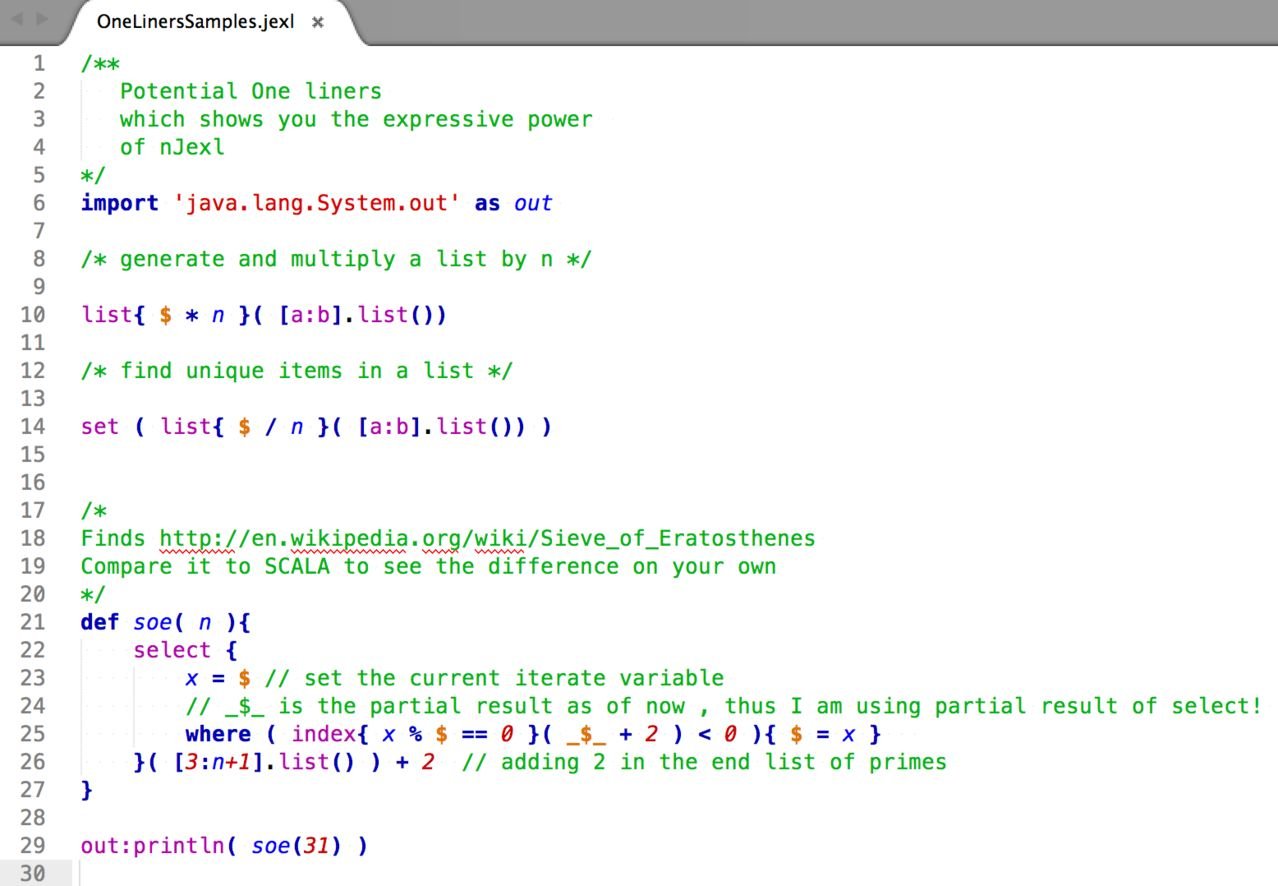
\includegraphics[scale=0.6]{sublime.jpeg}
\end{center}
\caption{Using Sublime Text}
\label{fig_2_1}
\end{figure}

To include for vim :

Create these two files :

\begin{lstlisting}[style=all]
    $HOME/.vim/ftdetect/jxl.vim
    $HOME/.vim/syntax/jxl.vim
\end{lstlisting}

For most \*nix systems it would be same as :

\begin{lstlisting}[style=all]
    mkdir -p ~/.vim/ftdetect/
    touch ~/.vim/ftdetect/jxl.vim 
    touch ~/.vim/syntax/jxl.vim 
\end{lstlisting}

Now on the \$HOME/.vim/ftdetect/jxl.vim  file, put this line :

\begin{lstlisting}[style=all]
    autocmd BufRead,BufNewFile *.jxl,*.jexl,*.njxl,*.njexl  set filetype=jxl
\end{lstlisting}

Note that you should not have blanks between commas.
And then, copy the content of the \href{https://github.com/nmondal/njexl/blob/master/doc/jxl.vim}{vim syntax file here} 
in the \$HOME/.vim/syntax/jxl.vim file as is.

If everything is fine, you can now open jexl scripts in vim!

\begin{figure}
\begin{center}
\leavevmode
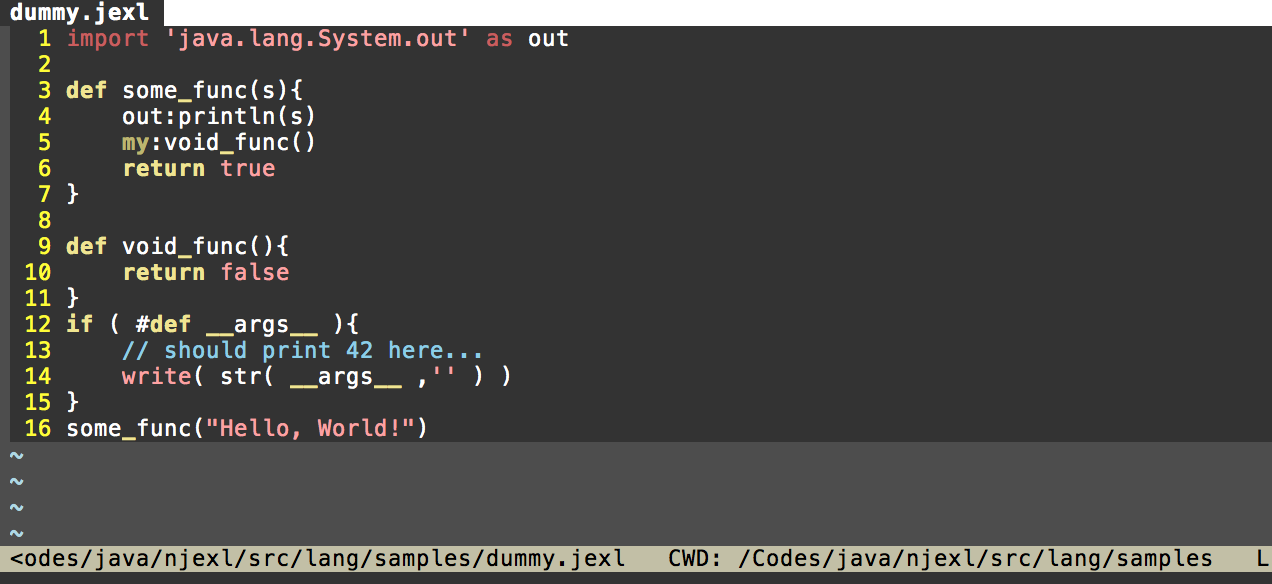
\includegraphics[scale=0.6]{vim.png}
\end{center}
\caption{Using Vim (MacVim)}
\label{fig_2_1}
\end{figure}


\end{subsection} 

\end{section}




 %complete
\chapter{nJexl Syntax in 3 Minutes}\label{intro-njexl}

{\LARGE W}ith some understanding on C,C++, Java, then it will be very easy for you to learn nJexl. The biggest syntactic difference between nJexl and other languages is that the ';' statement end character is optional. When we consider a nJexl program it can be defined as a collection of objects that communicate via invoking each others methods. 


\begin{section}{Building Blocks}

\begin{subsection}{Identifiers}
\index{identifiers}
nJexl is case-sensitive, which means identifier Hello and hello would have different meaning.
All nJexl components require names. Names used for objects, classes, variables and methods are called identifiers. 
A keyword cannot be used as an identifier and identifiers are case-sensitive. 
See here for a list of keywords. 

\end{subsection}


\begin{subsection}{Assignments}
\index{assignment}
Most basic syntax of nJexl is, like any other language : assignment.
\begin{lstlisting}[style=JexlStyle][float]
 a = 1 //  assigns local variable a to Integer 1
 b = 1.0 //assigns local variable a to b float 1.0
 c = 'Hello, nJexl' // assigns local variable c to String 'Hello, nJexl'
 d = "Hello, nJexl" ## same, strings are either single or double quoted 
 /* 
 assigns the *then* value of a to e, 
 subsequent change in a wont reflect in e 
 */
 e = a \end{lstlisting}

\end{subsection}

\begin{subsection}{Comments}
\index{comments}

See from the previous subsection "//" used as line comments. So is "\#\#".
Along with the multiline comment "/*" with  "*/" :

\end{subsection}


\begin{subsection}{Basic Types}

Basic types are :
\begin{lstlisting}[style=JexlStyle][float]
 a = 1 // Integer 
 b = 1.0 //  float 
 c = 'Hello, nJexl' // String 
 d = 1.0d ## Double 
 I = 1h // BigInteger 
 D = 1.0b // BigDecimal  
 tt = true // boolean 
 tf = false // boolean 
 null_literal = null // special null type
\end{lstlisting}

\end{subsection}

\begin{subsection}{Multiple Assignment}
nJexl supports multiple assignment. It has various usage:

\begin{lstlisting}[style=JexlStyle][float]
 a = 1 // Integer 
 b = 1.0 //  float 
 c = 'Hello, nJexl' // String 
 // instead, do this straight :
 #(a,b,c ) = [ 1 , 1.0 , 'Hello, nJexl' ]   
\end{lstlisting}
\end{subsection}
\end{section}

\begin{section}{operators}
\index{operators}


\begin{subsection}{Arithmetic}
\index{operators : Arithmetic}
\begin{lstlisting}[style=JexlStyle][float]
a = 1 + 1 // addition : a <- 2
z = 1 - 1 // subtraction : z <- 0
m = 2 * 3 // multiply : m <- 6
d = 3.0 / 2.0 // divide d <- 1.5   
x = 2 ** 10 // Exponentiation x <- 1024
y = -x // negation, y <- -1024 
r = 3 % 2 // modulo, r <- 1 
r = 3 mod 2 // modulo, r <- 1    
a += 1 // increment and assign 
z -= 1 // decrement and assign 
\end{lstlisting}

\end{subsection}

\begin{subsection}{Logical}
\index{operators : Logical}
\begin{lstlisting}[style=JexlStyle][float]
o = true or true // true , or operator 
o = true || true // same 
a = true and false // false , and operator 
a = true && false // false, and operator  
defined_a = #def a // true if a is defined, false otherwise
o = (10 != 20 ) // not, true 
o = not ( 10 = 20 ) // true 
o = 10 eq 20 // false
\end{lstlisting}

\end{subsection}


\begin{subsection}{Comparison}
\index{operators : Comparison}
\begin{lstlisting}[style=JexlStyle][float]
t = 10 < 20 // true, less than
t = 10 lt  20 // true , less than 
f = 10 > 20 // false, greater then 
f = 10 gt 20 // false, greater then 
t = 10 <= 10 // true, less than or equal to 
t = 10 le  10 // true , less than or equal to 
t = 10 >= 10 // true, greater then or equal to 
t = 10 ge 10 // true, greater then or equal to 
t = ( 10 == 10 ) // true, equal to 
t = ( 10 eq 10 ) // true, equal to 
f = ( 10 != 10 ) // false, not equal to 
f = ( 10 ne 10 ) // false, not equal to 
\end{lstlisting}

\end{subsection}

\begin{subsection}{Ternary}
\index{operators : Ternary}
\begin{lstlisting}[style=JexlStyle][float]
// basic ternary 
min = a < b ? a : b // general form (expression)?option1:option2 
// try fixing null with it
non_null = a == null? b : a
// or use the null coalescing operator   
non_null = a ?? b 
// same can be used as definition coalescing
defined = #def(a) ? a : b
//same as above 
defined = a ?? b
\end{lstlisting}

\end{subsection}


\end{section}


\begin{section}{Conditions}
\index{Conditionals}

People coming from any other language would find them trivial.

\begin{subsection}{If}
\index{Conditionals : if}

\begin{lstlisting}[style=JexlStyle][float]
x = 10 
if ( x < 100 ){
   x = x**2
}
write(x) // writes back x to standard output : 100
\end{lstlisting}
\end{subsection}

\begin{subsection}{Else}
\index{Conditionals : else}

\begin{lstlisting}[style=JexlStyle][float]
x = 1000 
if ( x < 100 ){
   x = x**2
}else{
  x = x/10 
}
write(x) // writes back x to standard output : 100
\end{lstlisting}
\end{subsection}

\begin{subsection}{Else If}
\index{Conditionals : else if}

\begin{lstlisting}[style=JexlStyle][float]
x = 100 
if ( x < 10 ){
   x = x**2
} else if( x > 80  ){
  x = x/10 
} else {
   x = x/100 
}
write(x) // writes back x to standard output : 10
\end{lstlisting}
\end{subsection}

\begin{subsection}{GoTo}
\index{Conditionals : jump, goto}

\begin{lstlisting}[style=JexlStyle][float]
/* 
 In case anyone like to use GOTO
*/
i = 0 
goto #label false // wont go there 
goto #label (i == 0) // will go there 
i = 2 
write("This should be skipped")

#label
write("This should be printed")
goto #unconditional
#unconditional
return i 
\end{lstlisting}
\end{subsection}
\end{section}

\begin{section}{Loops}
\index{Loops}

\begin{subsection}{While}
\index{Loops : while}

\begin{lstlisting}[style=JexlStyle][float]
i = 0 
while ( i < 42 ){
  write(i)
  i += 1
}
\end{lstlisting}

\end{subsection}

\begin{subsection}{For}
\index{Loops : for}

For can iterate over any iterable, 
in short, it can iterate over string, any collection of objects,
a list, a dictionary or a range.
That is the first type of for :
\index{Loops : for, range}
\begin{lstlisting}[style=JexlStyle][float]
for ( i : [0:42] ){ // [a:b] is a range type 
  write(i)
}
\end{lstlisting}
The result is the same as the while loop.
A standard way, from C/C++/Java is to write the same as in :
\index{Loops : for, conditioned}
\begin{lstlisting}[style=JexlStyle][float]
for ( i = 0 ; i < 42 ; i+= 1  ){ // [a:b] is a range type 
  write(i)
}
\end{lstlisting}
\end{subsection}
\end{section}

\begin{section}{Functions}
\index{functions}

\begin{subsection}{Defining}
\index{functions : define}

Functions are defined using the $def$ keyword.
And they can be assigned to variables, if one may wish to.
\begin{lstlisting}[style=JexlStyle][float]
def count_to_num(num){
   for ( i : [0:num] ){
      write(i)
   }
}
// just assign it 
fp = count_to_num
\end{lstlisting}

One can obviously return a value from function :

\begin{lstlisting}[style=JexlStyle][float]
def say_something(word){
   return ( "Hello " + word ) 
}
\end{lstlisting}
\end{subsection}

\begin{subsection}{Calling}
\index{functions : calling}

Calling a function is trivial :

\begin{lstlisting}[style=JexlStyle][float]
// calls the function with parameter
count_to_num(42) 
// calls the function at the variable with parameter
fp(42) 
// calls and assigns the return value 
greeting = say_something("Homo Erectus!" ) 
\end{lstlisting}

\end{subsection}

\begin{subsection}{Global Variables}
\index{global variables}
As you would be knowing that the functions create their local scope, 
so if you want to use variables - they must be defined in global scope.
Every external variable is readonly to the local scope, but to write to it, use $var$ keyword.  

\begin{lstlisting}[style=JexlStyle][float]
var a = 0
x = 0 
def use_var(){
   a = 42 
   write(a) // prints 42 
   write(x) // prints 0, can access global 
   x = 42 
   write(x) // prints 42 
}
// call the method
use_var()
write(a) // global a, prints 42 
write(x) // local x, prints 0 still
\end{lstlisting}
The result would be :
\begin{lstlisting}
42
0
42
42
0
\end{lstlisting}
\end{subsection}

\end{section}

\begin{section}{Anonymous Function as a Function Parameter}
\index{functions : anonymous}
A basic idea about what it is can be found \href{https://en.wikipedia.org/wiki/Anonymous\_function}{here}.
As most of the Utility functions use a specific type of anonymous function, 
which is nick-named as "Anonymous Parameter" to a utility function.

\begin{subsection}{Why it is needed?}

Consider a simple problem of creating a list from an existing one, 
by modifying individual elements in some way. This comes under 
\href{https://en.wikipedia.org/wiki/Map\_(higher-order\_function)}{map} , but the idea can be shared much simply:

\begin{lstlisting}[style=JexlStyle][float]
l = list()
  for ( x : [0:n] ){
      l.add ( x * x ) 
  }
return l 
\end{lstlisting}
Observe that the block inside the *for loop* takes minimal two parameters, 
in case we write it like this :
\begin{lstlisting}[style=JexlStyle][float]
// return is not really required, last executed line is return 
def map(x){ x * x } 
l = list()
for ( x : [0:n] ){
      l.add ( map(x) ) 
}
return l 
\end{lstlisting}

Observe now that we can now create another function, lets call it list\_from\_list :

\begin{lstlisting}[style=JexlStyle][float]
def map(x){ x * x } 
def list_from_list(fp, old_list)
    l = list()
    for ( x : old_list ){
    // use the function *reference* which was passed
      l.add( fp(x) )   
      }
      return l
} 
list_from_list(map,[0:n]) // same as previous 2 implementations
\end{lstlisting}
The same can be achieved in a much sorter way, with this :
\begin{lstlisting}[style=JexlStyle][float]
list{ $*$ }([0:n])
\end{lstlisting}

The curious block construct after the list function is called anonymous (function) parameter, 
which takes over the map function. The loop stays implicit, and the result is equivalent 
from the other 3 examples. The explanation is as follows.
For an anonymous function parameters, there are 3 implicit guaranteed arguments :

\begin{enumerate}
\item{ \$ --> Signifies the item of the collection , we call it the $ITEM$ }
\item{ \$\$ --> The context, or the collection itself , we call it the $CONTEXT$} 
\item{ \_ --> The index of the item in the collection, we call it the $ID$ of iteration } 
\item{ Another case to case parameter is :
     \_\$\_ --> Signifies the partial result of the processing , we call it $PARTIAL$ }
\end{enumerate}

\end{subsection}

\begin{subsection}{Some Use Cases}
The data structure section would showcase some use cases. 
But we would use a utility function to showcase the use of this anonymous function.
Suppose there is this function $minmax$ which takes a collection and returns the (min,max) tuple.
In short :

\begin{lstlisting}[style=JexlStyle][float]
#(min,max) = minmax(1,10,-1,2,4,11)
write(min) // prints -1
write(max) // prints 11    
\end{lstlisting}
But now, I want to find the minimum and maximum by length of a list of strings.
To do so, there has to be a way to pass the comparison done by length.
That is easy :

\begin{lstlisting}[style=JexlStyle][float]
#(min,max) = minmax{
             size($.0) < size($.1) 
             }( "" , "aa" , "abc" , "aa", "bbbbb" )
write(min) // prints empty string 
write(max) // prints bbbbb    
\end{lstlisting}

\end{subsection}

\end{section}

\begin{section}{Available Data Structures}

\begin{subsection}{Range}
\index{range}
A range is basically an iterable, with start and end separated by colon : $[a:b]$.
We already have seen this in action. "a" is inclusive while "b" is exclusive, 
this was designed the standard for loop in mind. There can also be an optional spacing parameter "s",
thus the range type in general is $[a:b:s]$, as described below:

\begin{lstlisting}[style=JexlStyle][float]
/* 
  when r = [a:b:s] 
  the equivalent for loop is :
  for ( i = a ; i < b ; i+= s ){
    ... body now ...  
  }
*/
r1 = [0:10] // a range from 0 to 9 with default spacing 1
//a range from 1 to 9 with spacing 2
r2 = [1:10:2] //1,3,5,7,9   
\end{lstlisting}
\end{subsection}

\begin{subsection}{Array}
\index{array()}

A very simple way to generate inline array is this:

\begin{lstlisting}[style=JexlStyle][float]
a1 = [0 , 1, 2, 3 ] // an integer array 
a2 = [1 , 2.0 , 3, 4 ] // a number array 
ao = [ 0 , 1, 'hi', 34.5 ] // an object array   
AO = array ( 0,1,2,3 ) // an object array  
\end{lstlisting}
Arrays are not modifiable, you can not add or remove items in an array.
But, you can replace them :
\begin{lstlisting}[style=JexlStyle][float]
a1[0] = 42 // now a1 : [ 42, 1, 2, 3 ]
\end{lstlisting}
\end{subsection}

\begin{subsection}{List}
\index{list()}

To solve the problem of adding and deleting item from an array, list were invented.
\begin{lstlisting}[style=JexlStyle][float]
l = list ( 0,1,2,3 ) // a list  
l += 10 // now the list is : 0,1,2,3,10
l -= 0 // now the list is : 1,2,3,10
x = l[0] // x is 1 now
l[1] = 100 // now the list is : 1,100,3,10 
\end{lstlisting}

\end{subsection}

\begin{subsection}{Set}
\index{set()}

A set is a list such that the elements do not repeat.
Thus :

\begin{lstlisting}[style=JexlStyle][float]
// now the set is : 0,1,2,3
s = set ( 0,1,2,3,1,2,3 ) // a set  
s += 5 // now the set is : 0,1,2,3,5 
s -= 0 // now the set is : 1,2,3
\end{lstlisting}
\end{subsection}

\begin{subsection}{Dict}
\index{dict()}

A dictionary is a collection ( a list of ) (key,value) pairs.
The keys are unique, they are the $keySet()$. Here is how one defines a dict:

\begin{lstlisting}[style=JexlStyle][float]
d1 = { 'a' : 1 , 'b' : 2 } // a dictionary   
d2 = dict( ['a','b'] , [1,2] ) // same dictionary  
x = d1['a'] // x is 1
x = d1.a // x is 1 
d1.a = 10 // now d1['a'] --> 10 
\end{lstlisting}

\end{subsection}

\end{section}

 %complete
\chapter{Formal Constructs}\label{using-predicates}

{\LARGE F}ormalism is the last thing that stays in a software developers mind nowadays. This is a result of mismanaging expectation - software may be art, but is not science at all. Most of the cases, a bit of formal thinking solves a lot of the problems that can come.
This section would be specifically to understand what sort of formalism we can use in practice.

\begin{section}{Conditional Building Blocks}

\begin{subsection}{Formalism}
In a formal logic like FOPL, the statements can be made from the basic ingredients, 
\emph{``there exist''} and \emph{``for all''}. We need to of course put some logical stuff like $AND$, $OR$,
and some arithmetic here and there, but that is what it is.

If we have noted down the \emph{sorting problem} in chapter 2, we would have restated the problem as :

\begin{center}
\emph{ There does not exist an element which is less than that of the previous one. }
\end{center} 

In mathematical logic, \emph{``there exists''} becomes : $\exists$ and \emph{``for all''} becomes $\forall$.
and logical not is shown as $\neg$ ,  So, the same formulation goes in : let $S = \{ 0, 1, 2, ... , size(a)-1  \} $, then :

$$
  i \in S ; \forall \; i  \neg \; ( \exists \; a[i] \; s.t. \; a[i] < a[i-1]    ) 
$$ 

And the precise formulation of what is a sorted array/list is done.

\end{subsection}


\begin{subsection}{There Exist In Containers}
To check, if some element is, in some sense exists inside a container ( list, set, dict, array, heap )
one needs to use the $IN$ operator, which is $@$. \index{operator : \@}

\begin{lstlisting}[style=JexlStyle][float]
l = [1,2,3,4] // l is an array 
in = 1 @ l // in is true 
in = 10 @ l // in is false 
d = { 'a' : 10 , 'b' : 20  }
in = 'a' @ d // in is true 
in = 'c' @ d // in is false 
in = 10 @ d // in is false 
in = 10 @ d.values() // in is true 
s = "hello"
in = "o" @ s // in is true 
\end{lstlisting}

This was not simply put in the place simply because we dislike $x.contains(y)$, in fact we do.
We dislike the form of object orientation where there is no guarantee that $x$ would be null or not.
Formally, then :

\begin{lstlisting}[style=JexlStyle][float]
// equivalent function 
def in_function(x,y){
   if ( empty(x) ) return false 
   return x.contains(y) 
}
// or one can use simply 
y @ x // same result
\end{lstlisting}
\end{subsection}

\begin{subsection}{Size of Containers : empty, size, cardinality}
To check whether a container is empty or not, 
use the $empty()$ \index{empty()} function, just mentioned above. Hence:
\begin{lstlisting}[style=JexlStyle][float]
n = null
e = empty(n) // true 
n = []
e = empty(n) // true 
n = list()
e = empty(n) // true 
d = { : }
e = empty(d) // true 
nn = [ null ]
e = empty(nn) // false 
\end{lstlisting}

For the actual size of it, there are two alternatives.
One is the $size()$ \index{size()}  function :

\begin{lstlisting}[style=JexlStyle][float]
n = null
e = size(n) // -1 
n = []
e = size(n) // 0 
n = list()
e = size(n) // 0 
d = { : }
e = size(d) // 0 
nn = [ null ]
e = size(nn) // 1 
\end{lstlisting}

Observe that it returns negative given input null. 
That is a very nice way of checking null.
The other one is the $cardinal$ operator \index{operator : \#\|\| }:

\begin{lstlisting}[style=JexlStyle][float]
n = null
e = #|n| // 0 
n = []
e = #|n| // 0 
n = list()
e = #|n| // 0 
d = { : }
e = #|d| // 0 
nn = [ null ]
e = #|nn| // 1 
\end{lstlisting}
This operator in some sense gives a measure. It can not be negative, 
so cardinality of $null$ is also 0. 
\end{subsection}

\begin{subsection}{There Exist element with Condition : index, rindex }
This pose a delicate problem. Given we have can say if \emph{``y in container x''} or not,
what if when asked a question like : \emph{ ``is there a y in x such that f(y) is true''} ?

Notice this is the same problem we asked about sorting. Is there an element (y) in x, 
such that the sorting order is violated? If not, the collection is sorted.
This brings back the $index$ function \index{index()}.
We are already familiar with the usage of $index()$ function from chapter 2.
But we would showcase some usage :

 
\begin{lstlisting}[style=JexlStyle][float]
l = [ 1, 2, 3, 4, 5, 6 ]
// search an element such that double of it is 6
i = index{ $ * 2 == 6 }(l) // i : 2 
// search an element such that it is between 3 and 5 
i = index{ $ < 5 and $ > 3 }(l) // i : 3 
// search an element such that it is greater than 42
i = index{  $ > 42 }(l) // i : -1, failed 
\end{lstlisting}

The way index function operates is: the statements inside the anonymous block are executed.
If the result of the execution is true, the index function returns the index in the collection.
If none of the elements matches the true value, it returns $-1$.
Index function runs from left to right, and there is a variation $rindex()$ \index{index()}
which runs from right to left.

\begin{lstlisting}[style=JexlStyle][float]
l = [ 1, 2, 3, 4, 5, 6 ]
// search an element such that it is greater than 3  
i = index{ $ > 3 }(l) // i : 3
// search an element such that it is greater than 3  
i = rindex{ $ > 3 }(l) // i : 5 
// search an element such that it is greater than 42
i = rindex{  $ > 42 }(l) // i : -1, failed 
\end{lstlisting}

Thus, the \emph{there exists} formalism is taken care by these operators and functions together.

\end{subsection}


\begin{subsection}{For All elements with Condition : select }
We need to solve the problem of \emph{for all}. This is done by $select()$ function \index{select()}.
The way select function works is : executes the anonymous statement block, and if the condition is true, 
then select and collect that particular element, and returns a list of collected elements.

\begin{lstlisting}[style=JexlStyle][float]
l = [ 1, 2, 3, 4, 5, 6 ]
// select all even elements 
evens = select{ $ % 2 == 0 }(l)
// select all odd elements 
odds = select{ $ % 2 == 1 }(l) 
\end{lstlisting}

\end{subsection}

\begin{subsection}{Partition a collection on Condition : partition }
Given a $select()$, we are effectively partitioning the collection into two halves,
$select()$ selects the matching partition. In case we want both the partitions, then 
we can use the $partition()$ function \index{partition()}.

\begin{lstlisting}[style=JexlStyle][float]
l = [ 1, 2, 3, 4, 5, 6 ]
#(evens,odds) = partition{ $ % 2 == 0 }(l)
write(evens) // prints 2, 4, 6 
write(odds) // prints 1, 3, 5
\end{lstlisting}
\end{subsection}

\begin{subsection}{Collecting value on Condition : where }
Given a $select()$ or $partition()$, we are collecting the values already 
in the collection. What about we want to change the values? 
This is done by the conditional known as $where()$ \index{where()}.
The way where works is, we put the condition inside the where.
The result would be the result of the condition, but the where clause body 
would be get executed. Thus, we can change the value we want to collect
by replacing the $ITEM$ variable, that is $\$$.

\begin{lstlisting}[style=JexlStyle][float]
l = [ 1, 2, 3, 4, 5, 6 ]
#(evens,odds) = partition{ where($ % 2 == 0){ $ = $**2  }  }(l)
write(evens) // prints 4, 16, 36 
write(odds) // prints 1, 3, 5
\end{lstlisting}

This is also called \emph{item rewriting} \index{item rewriting}.
\end{subsection}

\end{section}


\begin{section}{Operators from Set Algebra}

\begin{subsection}{Set Algebra}

Set algebra, in essence runs with the notions of the following ideas :
\begin{enumerate}
\item{There is an unique empty set.}
\item { The following operations are defined :
\begin{enumerate}{
     \item{Set Union is defined as : 
$$
U_{AB} = A \cup B \; :=  \{ x \in A \; or \; x \in B \} 
$$ 
}
    \item{Set Intersection is defined as : 
$$
I_{AB} = A \cap B \; :=  \{ x \in A \; and \; x \in B \} 
$$
}
\item{Set Minus is defined as : 
$$
M_{AB} = A \setminus B \; :=  \{ x \in A \; and \; x \not \in B \} 
$$
}
\item{Set Symmetric Difference is defined as : 
$$
\Delta_{AB} = ( A \setminus B ) \cup ( B  \setminus A ) 
$$
}
\item{Set Cross Product is defined as : 
$$
X_{AB} = \{ ( a, b ) \; | \; a \in A \; and \;  b \in B  \} 
$$
}
}
\end{enumerate}}
\item{ The following relations are defined:
\begin{enumerate}

\item{ Subset Equals :
$$
A \subseteq B \; when \;  x \in A \implies x \in B
$$
}

\item{ Equals :
$$
A = B \; when \; A \subseteq B \; and \; B \subseteq A
$$
}


\item{ Proper Subset :
$$
A \subset B \; when \; A \subseteq B \; and \; \exists x \in B \;s.t.\; x \not \in A
$$
}

\item{ Superset Equals:
$$
A \supseteq B \; when \; B \subseteq A 
$$
}

\item{ Superset :
$$
A \supset B \; when \; B \subset A 
$$
}
\end{enumerate}}
\end{enumerate}
\end{subsection}

\begin{subsection}{Set Operations on Collections}

For the sets, the operations are trivial.
\begin{lstlisting}[style=JexlStyle][float]
s1 = set(1,2,3,4)
s2 = set(3,4,5,6)
u = s1 | s2 // union is or : u = { 1,2,3,4,5,6}
i = s1 & s2 // intersection is and : i = { 3,4 }
m12 = s1 - s2 // m12 ={1,2}
m21 = s2 - s1 // m12 ={5,6}
delta = s1 ^ s2 // delta = { 1,2,5,6}
\end{lstlisting}

For the lists or arrays, where there can be multiple elements present, 
this means a newer formal operation.
Suppose in both the lists, an element `e' is present, in $n$ and $m$ times.
So, when we calculate the following :
\begin{enumerate}
\item{Intersection :
  the count of $e$ would be $min(n,m)$.
}
\item{Union :
  the count of $e$ would be $max(n,m)$.
}
\item{Minus :
  the count of $e$ would be $max(0,n-m)$.
}

\end{enumerate}
With this, we go on for lists:

\begin{lstlisting}[style=JexlStyle][float]
l1 = list(1,2,3,3,4,4)
l2 = list(3,4,5,6)
u = l1 | l2 // union is or : u = { 1,2,3,3,4,4,5,6}
i = l1 & l2 // intersection is and : i = { 3,4 }
m12 = l1 - l2 // m12 ={1,2,3,4}
m21 = l2 - l1 // m12 ={5,6}
delta = l1 ^ l2 // delta = { 1,2,3,4,5,6}
\end{lstlisting}

Now, for dictionaries, the definition is same as lists, 
because there the dictionary can be treated as a list of key-value pairs.
So, for one pair to be equal to another, both the key and the value must match.
Thus:

\begin{lstlisting}[style=JexlStyle][float]
d1 = {'a' : 10, 'b' : 20 , 'c' : 30 }
d2 = {'c' : 20 , 'd' : 40  }
// union is or : u = { 'a' : 10, 'b' : 20, 'c' : [ 30,20] , 'd' : 40  }
u = d1 | d2 
i = d1 & d2 // intersection is and : i = { : } 
m12 = d1 - d2 // m12 = d1 
m21 = d2 - d1 // m12 = d2
delta = d1 ^ d2 // delta = {'a' : 10, 'b' : 20, 'd': 40}
\end{lstlisting}
\end{subsection}


\begin{subsection}{Collection Relation Comparisons}
The operators are defined as such:
\begin{enumerate}
\item{ $A \subset B $ is defined as $A < B $  }
\item{ $A \subseteq B $ is defined as $A <= B $  }
\item{ $A \supset B $ is defined as $A > B $  }
\item{ $A \supseteq B $ is defined as $A >= B $  }
\item{ $A = B$ is defined as $A == B$  }
\end{enumerate}

Note that when collections can not be compared at all, 
it would return false to showcase that the relation fails.

So, we go again with sets:

\begin{lstlisting}[style=JexlStyle][float]
s1 = set(1,2,3)
s2 = set(1,3)
sub = s2 < s1 // true  
sup = s1 > s2 // true 
sube = ( s2 <= s1 ) // true  
supe = (s1 >= s2) // true 
s3 = set(5,6)
s1 < s3 // false 
s3 > s1 // false 
s1 != s3 // true
\end{lstlisting}

So, we go again with lists:

\begin{lstlisting}[style=JexlStyle][float]
l1 = list(1,2,3,3,4)
l2 = list(1,3,2)
sub = l2 < l1 // true  
sup = l1 > l2 // true 
sube = ( l2 <= l1 ) // true  
supe = (l1 >= l2) // true 
l3 = list(5,6)
l1 < l3 // false 
l3 > l1 // false 
l1 != l3 // true
\end{lstlisting}

And finally with dictionaries:

\begin{lstlisting}[style=JexlStyle][float]
d1 = {'a' : 10, 'b' : 20 , 'c' : 30 }
d2 = {'c' : 30 , 'a' : 10  }
sub = ( d2 < d1) // true 
sup = ( d1 > d2) // true
\end{lstlisting}
\end{subsection}

\begin{subsection}{Mixing Collections}
One can choose to intermingle $set$ with $list$, that promotes the $set$ to $list$.
Thus :

\begin{lstlisting}[style=JexlStyle][float]
s = set(1,2,3)
l = list(1,3,3,2)
sub = s < l  // true  
sup = l > s // true 
u = l | s // u = [1,2,3,3 ]
\end{lstlisting}

\end{subsection}

\end{section}


 %complete
\chapter{Comprehensions on Collections}\label{comprehension-collection}

{\LARGE C}omprehension is a method which lets one create newer collection from older ones.
In this chapter we would see how different collections can be made from existing collections.

\begin{section}{Using Anonymous Argument}

\begin{subsection}{Arrays and List}
The general form for list and arrays can be written ( as from chapter 2 ):
\begin{lstlisting}[style=JexlStyle][float]
def map(item) {/* does some magic */}
def comprehension(function, items){
   c = collection()
   for ( item : items ){
     c_m = function(c)
     c.add( c_m ) 
   }
   return c
}
//or this way :
c = collection{ function($) }(items)
\end{lstlisting}
Obviously $list()$ generates $list$ and $array()$ generates $array$.
Hence, these are valid :
\begin{lstlisting}[style=JexlStyle][float]
an = array{ $ + 2 }([1,2,3,4]) // [ 3,4,5,6 ]
ln = list{ $ ** 2 }([1,2,3,4]) // [1,4,9,16 ]
\end{lstlisting}

So, the result of the anonymous block is taken as a function to map the item into a newer item, 
and finally added to the final collection.

\end{subsection}

\begin{subsection}{Set}

Set also follows the same behavioural pattern just like $array()$ and $list()$, but one needs 
to remember that the $set$ collection does not allow duplicates. Thus:

\begin{lstlisting}[style=JexlStyle][float]
s = set{ $ % 3 }( [1,2,3,4,5] ) // [0,1,2]
\end{lstlisting}

Basically, the $map$ function for the $set$ construct, defines the key for the item.
Thus, unlike its cousins $list()$ and $array()$, the $set()$ function may return a collection
with size less than the input collection. 

\end{subsection}

\begin{subsection}{Dict}
Dictionaries are special kind of a collection with $(key,value)$ pair with unique keys.
Thus, creating a dictionary would mean uniquely specifying the key, value pair.
That can be specified either in a dictionary tuple way, or simply a pair way: 

\begin{lstlisting}[style=JexlStyle][float]
// range can be passed in for collection
d = dict{ t = { $ : $**2 }  }([0:4])
/* d = {0 : 0, 1 : 1, 2 : 4, 3:9 }  */
d = dict{ [ $ , $**2 ]  }([0:4]) // same as previous
\end{lstlisting}

There is another way of creating a dictionary, that is, 
passing two collections of same size, and making first collection 
as keys, mapping it to the corresponding second collection as values:

\begin{lstlisting}[style=JexlStyle][float]
k = ['a','b','c' ]
v = [1,2,3]
d = dict(k,v)
/*  d = { 'a' : 1 , 'b' : 2, 'c' : 3 }  */ 
\end{lstlisting}

\end{subsection}

\end{section}


\begin{section}{Alternate Iteration Flow Constructs}

\begin{subsection}{Continue and Break}
In normal iterative languages, there are continue and break.

The idea of continue would be as follows :
\begin{lstlisting}[style=JexlStyle][float]
for ( i : items ){
    if ( condition(i) ){
      // execute some 
      continue 
    }
    // do something else 
}
\end{lstlisting}
That is, when the condition is true, execute the code block, 
and then continue without going down further ( not going to do something else ). 

The idea of the break is :
\begin{lstlisting}[style=JexlStyle][float]
for ( i : items ){
    if ( condition(i) ){
      // execute some 
      break 
    }
    // do something else 
}
\end{lstlisting}
That is, when the condition is true, execute the code block, 
and then break without proceeding with the loop further. 
Evidently they change the flow of control of the iterations.
\end{subsection}

\begin{subsection}{Continue}
As we can see, the $condition()$ is implicit in both $break$ and $continue$,
in nJexl this has become explicit. Observe that:  

\begin{lstlisting}[style=JexlStyle][float]
for ( i : items ){
    continue( condition(i) ){ /* continue after executing this */} 
    // do something else 
}
\end{lstlisting}
is equivalent of what was being shown in the previous subsection.
As a practical example, lets have some fun with the problem of $FizzBuzz$,
that is, given a list of integers, if $n$ is divisible by $3$ print $Fizz$,
if something is divisible by $5$, print $Buzz$, and for anything else print the number $n$. 
A solution is :

\begin{lstlisting}[style=JexlStyle][float]
for ( n : integers ){
    continue( n % 15 ){ write('FizzBuzz') }
    continue( n % 3 ){ write('Fizz') }
    continue( n % 5 ){ write('Buzz') }
    write(n) 
}
\end{lstlisting}
Obviously, the block of the continue is optional.
Thus, one can freely code the way it was mentioned in the 
earlier subsection.
\end{subsection}


\begin{subsection}{Break}
As mentioned in the previous subsection, 
$break$ also has the same features as continue. 

\begin{lstlisting}[style=JexlStyle][float]
for ( i : items ){
    break( condition(i) ){ /* break loop after executing this */} 
    // do something else 
}
\end{lstlisting}
is equivalent of what was being shown in the previous subsection.
As a practical example, lets find if two elements of two lists
when added together generates a given value or not.
Formally :

$$
\exists (a,b) \in A \times B \; ; \; s.t. \; a + b = c  
$$

\begin{lstlisting}[style=JexlStyle][float]
A = [ 1, 4, 10, 3, 8 ]
B = [ 2, 11, 6 , 9 ]
c = 10 
for ( p : A*B  ){
    break( p[0] + p[1] ==  c ){ 
    write( '%d %d\n' , p[0] , p[1] ) } 
}
\end{lstlisting}
Obviously, the block of the break is optional.
\end{subsection}

\begin{subsection}{Substitute for Select}
One can readily use the $break$ and $continue$ in larger scheme of comprehensions.
Observe this :

\begin{lstlisting}[style=JexlStyle][float]
l_e1 = select{ $ % 2 == 0 }([0:10])
l_e2 = list{ continue($ % 2 != 0) ; $ }([0:10])
\end{lstlisting}
Both are the same list. Thus, a theoretical conversion rule is :

\begin{lstlisting}[style=JexlStyle][float]
ls = select{ <condition> }(collection)
lc = list{ continue( not ( <condition> ) ) ; $ }(collection)
\end{lstlisting}
now, the $ls == lc$, by definition.
More precisely, for a generic $select$ with $where$ clause:

\begin{lstlisting}[style=JexlStyle][float]
ls = select{ where ( <condition> ){ <body> } }(collection)
lc = list{ continue( not ( <condition> ) ) ; <body> }(collection)
\end{lstlisting}
Obviously, the $list$ function can be replaced with any $collection$ type : $array, set, dict$.

Similarly, $break$ can be used to simplify conditions :

\begin{lstlisting}[style=JexlStyle][float]
l_e1 = select{ $ % 2 == 0 and $ < 5 }([0:10])
l_e2 = list{ break( $ > 5 ) ;  continue($ % 2 != 0) ; $ }([0:10])
\end{lstlisting}

Note that Break body is inclusive:
  
\begin{lstlisting}[style=JexlStyle][float]
l = list{ break( $ > 3 ) { $ } ; $ }([0:10])
/* l = [ 1,2,3, 4] */
\end{lstlisting}
 
So, with a body, the boundary value is included into $break$.
\end{subsection}

\begin{subsection}{Uses of Partial}
One can use the $PARTIAL$ for using one one function to substitute another,
albeit loosing efficiency.
Below, we use list to create $effectively$ a set:

\begin{lstlisting}[style=JexlStyle][float]
l = list{ continue( $ @ _$_ ) ; $ }( [1,1,2,3,1,3,4] )
/* l = [ 1,2,3, 4] */
\end{lstlisting}

But it gets used properly in more interesting of cases.
What about finding the prime numbers using the Sieve of Eratosthenes?
We all know the drill imperatively:

\begin{lstlisting}[style=JexlStyle][float]
def is_prime( n ){
    primes = set(2,3,5)
    for ( x : [6:n+1] ){
        x_is_prime = true 
        for ( p : primes ) {
            break( x % p == 0  ){ x_is_prime = false }
        }
        if ( x_is_prime ){
          if ( x == n ) return true 
          primes += x 
        }
    }
    return false 
}
\end{lstlisting}
Now, a declarative style coding :

\begin{lstlisting}[style=JexlStyle][float]
def is_prime( n ){
    primes = set{
    // store the current number
        me = $
        // check : *me* is not prime - using partial set of primes
        not_prime_me = ( index{  me % $ == 0 }( _$_ ) >= 0 ) 
        // if not a prime, continue 
        continue( not_prime_me )
        // collect me, if I am prime 
        $   
    }( [2:n+1] )
    // simply check if n belongs to primes
    return ( n @ primes )  
}
\end{lstlisting}
Observe that, if we remove the comments, it is a one liner. 
It really is. Hence, declarative style is indeed succinct, and very powerful.

\end{subsection}

\end{section}



\begin{section}{Comprehensions using Multiple Collections : Join}

In the previous sections we talked about the comprehensions using a single collection.
But we know that there is this most general purpose comprehension, that is, 
using multiple collections. This section we introduce the $join()$ function.

\begin{subsection}{Formalism}
Suppose we have multiple sets $S_1,S_2,...S_n$.
Now, we want to generate this collection of tuples 
$$
e = <e_1,e_2,...,e_n> \; \in S_1 \times S_2 \times ... \times S_n
$$ 
such that the condition ( {https://en.wikipedia.org/wiki/Predicate\_(mathematical\_logic)}{predicate} ) $P(e) = true $.
This is what join really means. Formally, then :
$$
\{  e \in S_1 \times S_2 \times ... \times S_n \; | \; P(e) \} 
$$

\end{subsection}

\begin{subsection}{As Nested Loops}
Observe this, to generate a cross product of collection $A,B$, we must
go for nested loops like this:

\begin{lstlisting}[style=JexlStyle][float]
for ( a : A ){
   for ( b : B ) {
     write ( '(%s,%s)', a,b ) 
   }
}
\end{lstlisting}
This is generalised for a cross product of $A,B,C$, and generally into any cross product. 
Hence, the idea behind generating a tuple is nested loop.

Thus, the $join()$ operation with $condition()$ predicate essentially is :

\begin{lstlisting}[style=JexlStyle][float]
collect = collection()
for ( a : A ){
   for ( b : B ) {
      tuple = [a,b]
      if ( condition ( tuple ) ) { collect += tuple  } 
   }
}
\end{lstlisting}
\end{subsection}

\begin{subsection}{Join Function}
Observe that the free join, is really a full cross product, 
and is available using the power operator :

\begin{lstlisting}[style=JexlStyle][float]
A = ['a','b']
B = [ 0, 1 ]
j1 = A * B // [ [a,0] , [a,1] ,[b,0], [b,1] ]
j2 = join( A , B ) // [ [a,0] , [a,1] ,[b,0], [b,1] ]
\end{lstlisting}

But the power of $join()$ comes from the predicate expression one can pass in 
the anonymous block. Observe now, if we need 2 permutations of a list :

\begin{lstlisting}[style=JexlStyle][float]
A = ['a','b', 'c' ]
// generate 2 permutations 
p2 = join{  $.0 != $.1 } ( A , A,  A ) 
\end{lstlisting}
 
\end{subsection}

\begin{subsection}{Finding Permutations }
In the last subsection we figured out how to find 2 permutation.
The problem is when we move beyond 2, the condition can not be aptly specified as $\$.0 != \$.1 $.
It has to move beyond. So, for $^3P_3$ we have :

\begin{lstlisting}[style=JexlStyle][float]
A = ['a','b', 'c' ]
// generate 3 permutations 
p2 = join{ #|set($)| == #|$|  } ( A , A,  A ) 
\end{lstlisting}

which is the declarative form for permutation, given all elements are unique. 
\end{subsection}

\begin{subsection}{Searching for Addition Result }
In the last section we were searching for a tuple $t$ from two collections $A,B$,
such that $c = t.0 + t.1$. We did that using power and break, now 
we can do slightly better:

\begin{lstlisting}[style=JexlStyle][float]
A = [ 1, 4, 10, 3, 8 ] 
B = [ 2, 11, 6 , 9 ]
c = 10
v = join{ break( $.0 + $.1 == c) }(A,B) 
/* v := [[1,9]] */
\end{lstlisting}

which is the declarative form of the problem. 
\end{subsection}

\begin{subsection}{Finding Combinations}
We did find permutation. What about combinations?
What about we want to find combinations from 3 elements, 
taken 2 at a time? We observe that every combination is still a permutation.
So, once it qualified as a permutation, we need to check that if the pair
is in strictly increasing order or not (sorted). Thus :

\begin{lstlisting}[style=JexlStyle][float]
A = [ 'a' ,'b', 'c' ] 
c = join{ // check permutation , then 
       #|set($)| == #|$| and 
       // check sorted - same trick we used earlier too!      
       index{ _ > 0 and  $$[_-1] > $ }($) < 0 
    }(A,A)
\end{lstlisting}
This is how we can solve the problem with the aid of a declarative form. 
\end{subsection}

\end{section}



 %complete
\chapter{Types and Conversions}\label{type-conversions}

{\LARGE T}ypes are not much useful for general purpose programming, save that they avoid errors.
Sometimes they are necessary, and some types are indeed useful because they let us do 
many useful stuff. In this chapter we shall talk about these types and how to convert
one to another.

The general form for type casting can be written :
\begin{lstlisting}[style=JexlStyle][float]
val = type_function(value, optional_default_value = null )
\end{lstlisting}

How does this work? The system would try to cast $value$
into the specific type. If it failed, and there is no default value, 
it would return $null$. However, if default is passed, it would return 
that when conversion fails.
This neat design saves a tonnage of $try \; ... \; catch$ stuff. 

\begin{section}{Integer Family}
This section is dedicated to the natural numbers family.
We have :
\begin{enumerate}
\item{bool}
\item{short}
\item{char}
\item{int}
\item{long}
\item{INT : Java BigInteger}
\end{enumerate}

\begin{subsection}{Boolean}\index{bool()}
The syntax is :
\begin{lstlisting}[style=JexlStyle][float]
val = bool(value, optional_default_value = null )
val = bool(value, optional_matching_values[2])
\end{lstlisting}
Observe both in action :

\begin{lstlisting}[style=JexlStyle][float]
val = bool("hello") // val is null
val = bool("hello",false) // val is false
val = bool('hi', ['hi' , 'bye' ] ) // val is true 
val = bool('bye', ['hi' , 'bye' ] ) // val is false 
\end{lstlisting}

\end{subsection}

\begin{subsection}{Short}\index{short()}
This is almost never required, and is there for backward compatibility with Java data types.
The syntax is :

\begin{lstlisting}[style=JexlStyle][float]
val = short(value, optional_default_value = null )
\end{lstlisting}

Usage is :

\begin{lstlisting}[style=JexlStyle][float]
val = short("hello") // val is null
val = short("hello",0) // val is 0
val = short('42') // val is 42 
val = short(42) // val is 42 
\end{lstlisting}

\end{subsection}

\begin{subsection}{Character}\index{char()}
For almost all practical purposes, character is noting but the short value, 
interpreted by a code page.

The syntax is :

\begin{lstlisting}[style=JexlStyle][float]
val = char(value, optional_default_value = null )
\end{lstlisting}

Usage is :

\begin{lstlisting}[style=JexlStyle][float]
val = char("hello") // val is "h"
val = char(121231231,0) // val is 0
val = char('4') // val is '4' 
// ascii stuff?
val = char(65) // val is 'A'  
\end{lstlisting}

Generally none needs to get into this, because generally $String.charAt(index)$ is a good substitute
for finding a character.
\end{subsection}

\begin{subsection}{Integer}\index{int()}
This is very useful and the syntax is :

\begin{lstlisting}[style=JexlStyle][float]
val = int(value, optional_default_value = null )
\end{lstlisting}

Usage is :

\begin{lstlisting}[style=JexlStyle][float]
val = int("hello") // val is null
val = int("hello",0) // val is 0
val = int('42') // val is 42 
val = int(42) // val is 42 
val = int ( 10.1 ) // val is 10 
val = int ( 10.9 ) // val is 10 
\end{lstlisting}

\end{subsection}


\begin{subsection}{Long}\index{long()}
This is rarely required, and the syntax is :

\begin{lstlisting}[style=JexlStyle][float]
val = long(value, optional_default_value = null )
\end{lstlisting}

Usage is :

\begin{lstlisting}[style=JexlStyle][float]
val = long("hello") // val is null
val = long("hello",0) // val is 0
val = long('42') // val is 42 
val = long(42) // val is 42 
val = long( 10.1 ) // val is 10 
val = long( 10.9 ) // val is 10 
\end{lstlisting}

\end{subsection}

\begin{subsection}{BigInteger}\index{INT()}
This is sometimes required, and the syntax is :

\begin{lstlisting}[style=JexlStyle][float]
val = INT(value, base=10, default_value = null )
\end{lstlisting}

Usage is :

\begin{lstlisting}[style=JexlStyle][float]
val = INT("hello") // val is null
val = INT('hi',10,42 )// val is 42
val = INT('42') // val is 42 
val = INT(54,13 ) // val is 42 
\end{lstlisting}

\end{subsection}
\end{section}


\begin{section}{Rational Numbers Family}
This section is dedicated to the floating point numbers family.
We have :
\begin{enumerate}
\item{float}
\item{double}
\item{BigDecimal}
\end{enumerate}

\begin{subsection}{Float}\index{float()}
This is not very useful and the syntax is :

\begin{lstlisting}[style=JexlStyle][float]
val = float(value, optional_default_value = null )
\end{lstlisting}

Usage is :

\begin{lstlisting}[style=JexlStyle][float]
val = float("hello") // val is null
val = float("hello",0) // val is 0.0
val = float('42') // val is 42.0 
val = float(42) // val is 42.0 
val = float ( 10.1 ) // val is 10.1 
val = float ( 10.9 ) // val is 10.9 
\end{lstlisting}

\end{subsection}


\begin{subsection}{Double}\index{double()}
This is generally required, and the syntax is :

\begin{lstlisting}[style=JexlStyle][float]
val = double(value, optional_default_value = null )
\end{lstlisting}

Usage is :

\begin{lstlisting}[style=JexlStyle][float]
val = double("hello") // val is null
val = double("hello",0) // val is 0.0
val = double('42') // val is 42.0 
val = double(42) // val is 42.0 
val = double( 10.1 ) // val is 10.1 
val = double( 10.9 ) // val is 10.9 
\end{lstlisting}

\end{subsection}

\begin{subsection}{BigDecimal}\index{DEC()}
This is sometimes required, and the syntax is :

\begin{lstlisting}[style=JexlStyle][float]
val = DEC(value,default_value = null )
\end{lstlisting}

Usage is :

\begin{lstlisting}[style=JexlStyle][float]
val = DEC("hello") // val is null
val = DEC('hi',10,42 )// val is 42.0
val = DEC('42') // val is 42.0 
val = DEC(42.00001 ) // val is 42.00001
\end{lstlisting}

\end{subsection}

\end{section}

\begin{section}{The Chrono Family}
\index{date}\index{time}\index{instant}\index{format : date and time}

Handling date and time has been a problem, that too with timezones.
nJexl simplifies the stuff. 
We have three basic types to handle date/time:
\begin{enumerate}
\item{date : $java.lang.Date$ : because of Java compatibility with SDKs. }
\item{time : $org.joda.time.DateTime$ : that is the best one out there. }
\item{instant : $java.time.Instant$ : for newer systems who wants to experiment. }
\end{enumerate}


\begin{subsection}{Date}\index{date()}
This is how you create a date:
\begin{lstlisting}[style=JexlStyle][float]
val = date([ value, date_format ] )
\end{lstlisting}

With no arguments, it gives the current date time:

\begin{lstlisting}[style=JexlStyle][float]
today = date()
\end{lstlisting}

The default date format is $yyyyMMdd$, so :
\begin{lstlisting}[style=JexlStyle][float]
dt = date('20160218') // Thu Feb 18 00:00:00 IST 2016
\end{lstlisting}

For all the date formats on dates which are supported, 
see \href{https://docs.oracle.com/javase/8/docs/api/java/text/SimpleDateFormat.html}{SimpleDateFormat}.

Take for example :

\begin{lstlisting}[style=JexlStyle][float]
dt = date('2016/02/18', 'yyyy/MM/dd' ) // Thu Feb 18 00:00:00 IST 2016
dt = date('2016-02-18', 'yyyy-MM-dd' ) // Thu Feb 18 00:00:00 IST 2016
\end{lstlisting}


\end{subsection}

\begin{subsection}{Time}\index{time()}

This is how you create a joda \href{http://joda-time.sourceforge.net/apidocs/org/joda/time/DateTime.html}{DateTime}:
\begin{lstlisting}[style=JexlStyle][float]
val = time([ value, date_format , time_zone] )
\end{lstlisting}

With no arguments, it gives the current date time:

\begin{lstlisting}[style=JexlStyle][float]
today = time()
\end{lstlisting}

The default date format is $yyyyMMdd$, so :
\begin{lstlisting}[style=JexlStyle][float]
dt = time('20160218') // 2016-02-18T00:00:00.000+05:30
\end{lstlisting}

For all the date formats on dates which are supported, 
see \href{http://www.joda.org/joda-time/apidocs/org/joda/time/format/DateTimeFormat.html}{DateTimeFormat}.

Take for example :

\begin{lstlisting}[style=JexlStyle][float]
dt = time('2016/02/18', 'yyyy/MM/dd' ) // 2016-02-18T00:00:00.000+05:30
dt = time('2016-02-18', 'yyyy-MM-dd' ) // 2016-02-18T00:00:00.000+05:30
\end{lstlisting}

If you want to convert one time to another timezone, you need to give the time, 
and the \href{http://joda-time.sourceforge.net/timezones.html}{timezone}:

\begin{lstlisting}[style=JexlStyle][float]
dt = time()
dt_honolulu = time(dt , 'Pacific/Honolulu' ) // 2016-02-17T17:23:02.754-10:00 
dt_ny = time( dt, 'America/New_York' ) // 2016-02-17T22:23:02.754-05:00
\end{lstlisting}

\end{subsection}


\begin{subsection}{Instant}\index{instant()}

With no arguments, it gives the current instant time:

\begin{lstlisting}[style=JexlStyle][float]
today = instant()
\end{lstlisting}

It is freely mixable with other chrono types.

\end{subsection}


\begin{subsection}{Comparison on Chronos}\index{operator : compare, chrono }
All these date time types are freely mixable, 
and all comparison operations are defined with them.
Thus :

\begin{lstlisting}[style=JexlStyle][float]
d = date() // wait for some time 
t = time() // wait for some time 
i = instant()
// now compare 
c = ( d < t and t < i ) // true 
c = ( i > t and t > d ) // true 
\end{lstlisting}

Tow dates can be equal to one another, but not two instances,
that is a very low probability event, almost never.
Thus, equality makes sense when we know it is date, and not instant :

\begin{lstlisting}[style=JexlStyle][float]
d = date('19470815') // Indian Day of Independence  
t = time('19470815') // Indian Day of Independence  
// now compare 
c = ( d == t ) // true 
\end{lstlisting}

\end{subsection}

\begin{subsection}{Arithmetic on Chronos}
\index{arithmetic : chorono}
Dates, obviously can not be multiplied or divided.
That would be a sin. However, dates can be added with other reasoanable values, 
dates can be subtracted from one another, and $time()$ can be added or subtracted by days, months or even year.
More of what all date time supports, 
see the manual of \href{http://joda-time.sourceforge.net/apidocs/org/joda/time/DateTime.html}{DateTime}.

To add time to a date, there is another nifty method :

\begin{lstlisting}[style=JexlStyle][float]
d = date('19470815') // Indian Day of Independence  
time_delta_in_millis = 24 * 60 * 60 * 1000 // next day 
nd = date( d.time + time_delta_in_millis ) // Sat Aug 16 00:00:00 IST 1947 
\end{lstlisting}

Same can easily be achived by the $plusDays()$ function :

\begin{lstlisting}[style=JexlStyle][float]
d = time('19470815') // Indian Day of Independence  
nd = nd.plusDays(1) // 1947-08-16T00:00:00.000+05:30 
\end{lstlisting}
\end{subsection}

\end{section}

\begin{section}{String : Using str}
\index{str()}
Everything is just a string. It is. Thus every object should be able to be converted to and from out of strings.
Converting an object to a string representation is called \href{https://en.wikipedia.org/wiki/Serialization}{Serialization},
and converting a string back to the object format is called \emph{DeSerialization}.
This is generally done in nJexl by the function $str()$.

\begin{subsection}{Null}
$str()$ never returns null, by design. Thus:
\begin{lstlisting}[style=JexlStyle][float]
s = str(null)
s == 'null' // true  
\end{lstlisting}
\end{subsection}


\begin{subsection}{Integer}
\index{str : int,INT}
For general integers family, $str()$ acts normally. However, it takes overload
in case of $INT()$ or $BigInteger$ :
\begin{lstlisting}[style=JexlStyle][float]
bi = INT(42)
s = str(bi) // '42'
s = str(bi,2) // base 2 representation : 101010
\end{lstlisting}
\end{subsection}

\begin{subsection}{Floating Point}
\index{str : float,double,DEC}
For general floating point family, $str()$ acts normally. 
However, it takes overload, which is defined as :

\begin{lstlisting}[style=JexlStyle][float]
precise_string = str( float_value, num_of_digits_after_decimal )
\end{lstlisting}

To illustrate the point:

\begin{lstlisting}[style=JexlStyle][float]
d = 101.091891011
str( d, 0 ) // 101 
str(d,1) // 101.1  
str(d,2) // 101.09 
str(d,3) // 101.092 
\end{lstlisting}

\end{subsection}

\begin{subsection}{Chrono}
\index{str : date,time,instant }
Given a chrono family instance, $str()$ can convert them to a format of your choice.
These formats have been already discussed earlier, here they are again:
\begin{enumerate}
\item{Date : \href{https://docs.oracle.com/javase/8/docs/api/java/text/SimpleDateFormat.html}{SimpleDateFormat} }
\item{Time : \href{http://www.joda.org/joda-time/apidocs/org/joda/time/format/DateTimeFormat.html}{DateTimeFormat} }
\end{enumerate}

The syntax is :

\begin{lstlisting}[style=JexlStyle][float]
formatted_chrono = str( chrono_value , chrono_format )
\end{lstlisting}

Now, some examples :

\begin{lstlisting}[style=JexlStyle][float]
d = date()
t = time()
i = instant()
str( d ) // default is 'yyyyMMdd' : 20160218
str( t , 'dd - MM - yyyy' ) // 18 - 02 - 2016
str( i , 'dd-MMM-yyyy' ) // 18-Feb-2016 
\end{lstlisting}

\end{subsection}

\begin{subsection}{Collections}
\index{ str : collections }
Collections are formatted by str by default using `,'.
The idea is same for all of the collections, thus we would simply showcase some:

 


\end{subsection}

\begin{subsection}{Generalized $toString()$ }
\end{subsection}


\end{section}

























 %complete
%\chapter{Reusing Code}\label{code-reuse}

{\LARGE T}he tenet of nJexl is : \emph{``write once, forget''}.
That essentially means that the code written has to be sufficiently robust.
It also means that, we need to rely upon code written by other people.

How does this work? The system must be able to reuse $any$ code 
from Java SDK, and should be able to use any code that we ourselves wrote.
This chapter would be elaborating on this.

\begin{section}{The Import Directive}
\index{import}

\begin{subsection}{Syntax}

Most of the languages choose to use a non linear, tree oriented import.
nJexl focuses on minimising pain, so the import directive is linear.
The syntax is simple enough :
\index{import : java}
\begin{lstlisting}[style=JexlStyle]
import 'import_path' as unique_import_identifer
\end{lstlisting}

The directive imports the $stuff$ specified in the $import\_path$ and create 
an alias for it, which is : \\ \emph{unique\_import\_identifer},
Thus, there is no name collision at all in the imported script.
This \emph{unique\_import\_identifer} is known as the namespace.
\index{namespace}

\end{subsection}

 
\begin{subsection}{Examples}

Observe, if you want to import the class $java.lang.Integer$ :

\begin{lstlisting}[style=JexlStyle]
import 'java.lang.Integer' as Int
\end{lstlisting}

This directive would import the class, and create an alias which is $Int$.
To use this class further, now, we should be using :

\begin{lstlisting}[style=JexlStyle]
Int:parseInt('20') // int : 20
Int:valueOf('20') // int : 20 
\end{lstlisting}

In the same way, one can import an nJexl script :
\index{import : nJexl Script}

\begin{lstlisting}[style=JexlStyle]
// w/o any extension it would find the script automatically 
import 'from/some/folder/awesome' as KungFuPanda
// call a function in the script 
KungFuPanda:showAwesomeness()
\end{lstlisting}

\end{subsection}
 
\end{section}

\begin{section}{Using Existing Java Classes}

\begin{subsection}{Load Jar and Create Instance}
\index{import : load()}
The example of outer class, or rather a proper class 
has been furnished already. So, we would try to import a class
which is not there in the $CLASS\_PATH$ at all.

\begin{lstlisting}[style=JexlStyle]
// put all dependencies of xmlbeans.jar in there
success = load('path/to/xmlbeans_jar_folder') // true/false 
import 'org.apache.xmlbeans.GDate' as AGDate
\end{lstlisting}

Once we have this class now, we can choose to instantiate it,
See the manual of this class \href{https://xmlbeans.apache.org/docs/2.1.0/reference/org/apache/xmlbeans/GDate.html}{here}:

\index{new()}
\begin{lstlisting}[style=JexlStyle]
//create the class instance : use new() 
gd1 = new ( AGDate, date() )
// 2016-02-18T21:13:19+05:30
// or even this works 
gd2 = new ( 'org.apache.xmlbeans.GDate' , date() )
// 2016-02-18T21:13:19+05:30
\end{lstlisting}

And thus, we just created a Java class instance.
This is how we call Java objects, in general from nJexl.

Calling methods now is easy:

\begin{lstlisting}[style=JexlStyle]
cal = gd1.getCalendar() // calls a method 
/* 2016-02-18T21:13:19+05:30 */
\end{lstlisting}

Note that thanks to the way nJexl works, a method of the form $getXyz$
is equivalent to a field call $xyz$ so :

\begin{lstlisting}[style=JexlStyle]
cal = gd1.calendar // calls the method but like a field! 
/* 2016-02-18T21:13:19+05:30 */
\end{lstlisting}

\end{subsection}


\begin{subsection}{Import Enum}
\index{import : enum}\index{enum()}
Enums can be imported just like classes.
However, to use one, one should use the $enum()$ function:

\begin{lstlisting}[style=JexlStyle]
// creates a wrapper for the enum 
e = enum('com.noga.njexl.lang.extension.SetOperations')
// the enum value access using name 
value = e.OVERLAP
// using integer index 
value = e[4] 
\end{lstlisting}

The same thing can be achieved by :

\begin{lstlisting}[style=JexlStyle]
// gets the value for the enum 
v = enum('com.noga.njexl.lang.extension.SetOperations', 'OVERLAP' )
v = enum('com.noga.njexl.lang.extension.SetOperations', 4 )
\end{lstlisting}

\end{subsection}



\begin{subsection}{Import Static Field}
\index{import : static field}

Import lets you import static fields too. For example :

\begin{lstlisting}[style=JexlStyle]
// put all dependencies of xmlbeans.jar in there
import 'java.lang.System.out' as OUT
// now call println 
OUT.println("Hello,World") // prints it!
\end{lstlisting}

However, another way of achieving the same is :

\begin{lstlisting}[style=JexlStyle]
// put all dependencies of xmlbeans.jar in there
import 'java.lang.System' as SYS
// now call println 
SYS.out.println("Hello,World") // prints it!
// something like reflection
SYS['out'].println("Hello,World") // prints it!
\end{lstlisting}

\end{subsection}

\begin{subsection}{Import Inner Class or Enum}
\index{import : inner class, inner enum}
Inner classes can be accessed with the "\$" separator.
For example, observe from the SDK code of 
\href{http://grepcode.com/file/repository.grepcode.com/java/root/jdk/openjdk/8u40-b25/java/util/HashMap.java/}{HashMap},
that there is this inner static class $EntrySet$. So to import that:

\begin{lstlisting}[style=JexlStyle]
// note that $ symbol for the inner class
import 'java.util.HashMap$EntrySet' as ES
\end{lstlisting}

\end{subsection}

\end{section}

\begin{section}{Using nJexl Scripts}

We have already discussed how to import an nJexl script, 
so in this section we would discuss how to create a re-usable script.

\begin{subsection}{Creating a Script}
We start with a basic script, let's call it $hello.jxl$ :

\begin{lstlisting}[style=JexlStyle]
/* hello.jxl */
def say_hello(arg){
   write('Hello, ' + str(arg) )
}
s = "Some one"
my:say_hello(s)
/* end of script */
\end{lstlisting}
\index{namespace : my}
This script is ready to be re-used.
Observe that the function, when the script calls it, 
comes with the namespace $my:$, which says that, 
use current scripts $say\_hello()$ function.

\end{subsection}


\begin{subsection}{Relative Path}
\index{import : relative}
Suppose now we need to use this script, from another script, 
which shares the same folder as the ``hello.jxl''. 
Let's call this script $caller.jxl$. So, to import 
``hello.jxl'' in $caller.jxl$ we can do the following :

\begin{lstlisting}[style=JexlStyle]
import './hello.jxl' as Hello
\end{lstlisting}
   
but, the issue is when the runtime loads it, 
the relative path would with respect to the runtimes 
run directory. So, relative path, relative to the caller
would become a mess. To solve this problem, relative import is invented.

\begin{lstlisting}[style=JexlStyle]
import '_/hello.jxl' as Hello
Hello:say_hello('Waseem!" ) 
\end{lstlisting}

In this scenario, the runtime notices the ``$\_$'', and 
starts looking from the directory the $caller.jxl$ was loaded!    
Thus, without any $PATH$ hacks, the nJexl system works perfectly fine.

\end{subsection}

\begin{subsection}{Calling Functions}
\index{import : function call}

Functions can be called by using the namespace identifier, the syntax is :

\begin{lstlisting}[style=JexlStyle]
import 'some/path/file' as NS
NS:function(args,... ) 
\end{lstlisting}

If one needs to call the whole script, as a function, 
that is also possible, and that is done using the $\_\_me\_\_$ directive:

\begin{lstlisting}[style=JexlStyle]
import 'some/path/file' as NS
NS:__me__(args,... ) 
\end{lstlisting}
We will get back passing arguments to a function in a later chapter.
But in short, to call $hello.jxl$, as a function, the code would be :
\index{import : script as function}

\begin{lstlisting}[style=JexlStyle]
import '_/hello.jxl' as Hello
Hello:__me__() 
\end{lstlisting}

\end{subsection}


\end{section}

 %complete
%\chapter{Functional Style}\label{functional-style}

{\LARGE F}unctional style is a misnomer, in essence it boils down to some tenets:
\index{functional style}
\begin{enumerate}
\item{ Functions as first class citizens, they can be used as variables. }
\item{ Avoid modifying objects by calling methods on them. Only method calls returning create objects. }
\item{ Avoid conditional statements, replace them with alternatives. }
\item{ Avoid explicit iteration, replace them with recursion or other 
\href{https://en.wikipedia.org/wiki/Higher-order_function}{higher order functions}. }
\end{enumerate}


\begin{section}{Functions : In Depth}

As the functional style is attributed to functions, in this section
we would discuss functions in depth.

\begin{subsection}{Function Types}
nJexl has 3 types of functions.
\begin{enumerate}
\item{Explicit Functions :
\index{function : explicit}
This functions are defined using the $def$ keywords.
They are the $normal$ sort of functions, which everyone is aware of.
As an example take this :

\begin{lstlisting}[style=JexlStyle]
def my_function( a, b ){ a + b }
\end{lstlisting}
}

\item{Anonymous Functions :
\index{function : anonymous}
This functions are defined as a side-kick to another function, 
other languages generally calls them Lambda functions, but they do very specific 
task, specific to the host function. 
All the collection comprehension functions takes them :
\begin{lstlisting}[style=JexlStyle]
l = list { $** 2}([0:10] )
\end{lstlisting}
}

\item{Implicit Functions :
\index{function : implicit}
This functions are not even functions, they are the whole script body, 
to be treated as functions. Importing a script and calling it 
as a function qualifies as one : 
\begin{lstlisting}[style=JexlStyle]
import 'foo' as FOO
FOO:__me__()
\end{lstlisting}
}
\end{enumerate}

\end{subsection}

\begin{subsection}{Default Parameters}
\index{function : default parameters}

Every defined function in nJexl is capable of taking default values
for the parameters. For example :

\begin{lstlisting}[style=JexlStyle]
// default values passed 
def my_function( a = 40 , b = 2 ){ a + b }
// call with no parameters :
write ( my_function() ) // prints 42 
write ( my_function(10) ) // prints 12 
write ( my_function(1,2) ) // prints 3 
\end{lstlisting}
Note that, one can not mix the default and non default arbitrarily.
That is, all the default arguments must be specified from the right side.
Thus, it is legal :
\begin{lstlisting}[style=JexlStyle]
// one of the default values passed 
def my_function( a, b = 2 ){ a + b }
\end{lstlisting}
But it is not :
\begin{lstlisting}[style=JexlStyle]
// default values passed in the wrong order
def my_function( a = 10 , b ){ a + b }
\end{lstlisting}
\end{subsection}

\begin{subsection}{Named Arguments}
\index{functions : named args } 
In nJexl, one can change the order of the parameters passed, 
provided one uses the named arguments.
See the example:

\begin{lstlisting}[style=JexlStyle]
def my_function( a , b  ){ write('(a,b) = (%s ,%s)\n' ,a , b ) }
my_function(1,2)  // prints (a,b) = (1,2) 
my_function(b=11,a=10) //  prints (a,b) = (10,11) 
\end{lstlisting}
Note that, named args can not be mixed with unnamed args,
that is, it is illegal to call the method this way :

\begin{lstlisting}[style=JexlStyle]
// only one named values passed 
my_function(b=11,10) //  illegal 
\end{lstlisting}

\end{subsection}


\begin{subsection}{Arbitrary Number of Arguments}
\index{function : \_\_args\_\_ }\index{ function : arbitrary no. of args }
Every nJexl function can take arbitrary no of arguments.
To access the arguments, one must use the $\_\_args\_\_$ construct, as shown :
\begin{lstlisting}[style=JexlStyle]
// this can take any no. of arguments 
def my_function(){ 
   // access the arguments, they are collection  
   s = str (  __args__ , '#' )
   write(s)  
}
my_function(1,2,3,4)
/* prints 1#2#3#4 */
\end{lstlisting}

This means that, when a function expects $n$
parameters, but is only provided with $m < n $ parameters,
the rest of the expected  parameters not passed is passed as $null$.
\index{function : unassigned parameters}

\begin{lstlisting}[style=JexlStyle]
// this can take any no. of arguments, but named are 3 
def my_function(a,b,c){ 
   // access the arguments, they are collection  
   s = str (  __args__ , '#' )
   write(s)  
}
my_function(1,2)
/* prints 1#2#null */
\end{lstlisting}

In the same way when a function expects $n$
parameters, but is provided with $m > n $ parameters,
the rest of the passed  parameters can be accessed by the $\_\_args\_\_$ construct
\index{function : excess parameters} which was the first example.

Given we do not know in advance how many parameters will be passed 
to a script, the scripts, when used as functions must use this construct
as follows :

\begin{lstlisting}[style=JexlStyle]
/* I am a script  */
def main(){
 //  process args ...
}
/*
 only when this is defined, I am a script
 but being called as a function 
*/
if ( #def __args__ ) {
   x = __args__ // relocate 
   main( __args__ = x )
}
\end{lstlisting}
\end{subsection}

\begin{subsection}{Arguments Overwriting}

How to generate permutations from a list of object with 
$ ^nP_r$ ? Given a list $l$ of size $3$ We did $ ^3P_3$ :
\index{permutation}
\begin{lstlisting}[style=JexlStyle]
l = ['a','b','c' ]
perm_3_from_3 = join{ #|set($)| == #|$| }(l,l,l)
l = ['a','b','c' ,'d' ]
perm_4_from_4 = join{ #|set($)| == #|$| }(l,l,l,l)
perm_2_from_4 = join{ #|set($)| == #|$| }(l,l)
\end{lstlisting}
Thus, how to generate the general permutation?
As we can see, the arguments to the permutation 
is always varying. To fix this problem, 
\emph{argument overwriting} was invented.
That, in general, all the arguments to a function 
can be taken in runtime from a collection.
\index{function : argument overwriting}

\begin{lstlisting}[style=JexlStyle]
l = ['a','b','c' ,'d' ]
// this call overwrites the args :
perm_2_from_4 = join{ #|set($)| == #|$| }(__args__ = [l,l] )
\end{lstlisting}

Thus, to collect and permutate $r$ elements from a list $l$ is :
 
\begin{lstlisting}[style=JexlStyle]
perm_r = join{ #|set($)| == #|$| }(__args__ = array{ l }([0:r])  )
\end{lstlisting}

and we are done. This is as declarative as one can get.

\end{subsection}

\begin{subsection}{Recursion}
\index{function : recursion}
It is customary to introduce recursing with \href{https://en.wikipedia.org/wiki/Factorial}{factorial}.
We would not do that, we would introduce the concept delving the very heart of the foundation of mathematics, 
by introducing \href{https://en.wikipedia.org/wiki/Peano_axioms}{Peano Axioms}.
\index{function : Peano Axioms}
Thus, we take the most trivial of them all : Addition is a function that maps two natural numbers (two elements of N) to another one. 
It is defined recursively as:

\begin{lstlisting}[style=JexlStyle]
/* successor function */
def s( n ){
    if ( n == 0 ) return 1 
    return  ( s(n-1) + 1 )  
}
/* addition function */
def add(a,b){
  if ( b == 0 ) return a
  return s ( add(a,b-1) )
}
\end{lstlisting}

These functions do not only show the trivial addition in a non trivial manner, 
it also shows that the natural number system is recursive.
Thus, a system is recursive if and only if it is in 1-1 correspondence with the natural number system.
Observe that the addition function does not even have any addition symbol anywhere!

Now we test the functions:

\begin{lstlisting}[style=JexlStyle]
write(s(0)) // prints 1 
write(s(1)) // prints 2
write(s(5)) // prints 6
write(add(1,0)) // prints 1
write(add(1,5)) // prints 6
write(s(5,1)) // prints 6
\end{lstlisting}

Now, obviously we can do factorial :
\index{factorial}
\begin{lstlisting}[style=JexlStyle]
def fact(n){
   if ( n <= 0 ) return 1 
   return n * fact( n - 1 )
}
\end{lstlisting}

\end{subsection}

\begin{subsection}{Closure}
\index{function : closure}

A \href{https://en.wikipedia.org/wiki/Closure_(computer_programming)}{closure} 
is a function, whose return value depends on the value of one or more variables declared outside this function. 
Consider the following piece of code with anonymous function:

\begin{lstlisting}[style=JexlStyle]
multiplier = def(i) { i * 10 }
\end{lstlisting}

Here the only variable used in the function body, $i * 0$, is $i$, which is defined as a parameter to the function. 
Now let us take another piece of code:

\begin{lstlisting}[style=JexlStyle]
multiplier = def (i) {  i * factor } 
\end{lstlisting}

There are two free variables in multiplier: $i$ and $factor$. One of them, $i$, is a formal parameter to the function. 
Hence, it is bound to a new value each time multiplier is called. 
However, $factor$ is not a formal parameter, then what is this? 
Let us add one more line of code:

\begin{lstlisting}[style=JexlStyle]
factor = 3
multiplier = def (i) {  i * factor } 
\end{lstlisting}

Now, factor has a reference to a variable outside the function but in the enclosing scope. Let us try the following example:

\begin{lstlisting}[style=JexlStyle]
  write ( multiplier(1) ) // prints 3 
  write ( multiplier(14) ) // prints 42 
\end{lstlisting}
  
Above function references factor and reads its current value each time. 
If a function has no external references, then it is trivially closed over itself. No external context is required.

\end{subsection}

\begin{subsection}{Partial Function}
\index{function : nested, partial}
Partial functions are functions which lets one implement closure, w/o 
getting into the global variable way. Observe :

\begin{lstlisting}[style=JexlStyle]
// this shows the nested function 
def func(a){
    // here it is : note the name-less-ness of the function
    r = def(b){ // which gets assigned to the variable "r"
       write("%s + %s ==> %s\n", a,b,a+b)
    }
    return r // returning a function 
}
// get the partial function returned 
x = func(4)
// now, call the partial function 
x(2)
//finally, the answer to life, universe and everything :
x = func("4")
x("2")
\end{lstlisting}
This shows nested functions, as well as partial function.
\end{subsection}

\begin{subsection}{Functions as Parameters : Lambda}
\index{function : as parameter, lambda }

From the theory perspective, lambdas are defined in \href{https://en.wikipedia.org/wiki/Lambda_calculus}{Lambda Calculus}. 
As usual, the jargon guys made a fuss out of it, but as of now, we are using lambdas all along, for example :

\begin{lstlisting}[style=JexlStyle]
list{ $** 2 }(1,2,3,4)
\end{lstlisting}
 
The $\{ \$ ** 2 \}$ is a lambda. The parameter is implicit albeit, because it is meaningful that way. However, sometimes we need to pass named parameters. Suppose I want to create a function composition, first step would be to apply it to a single function :

\begin{lstlisting}[style=JexlStyle]
 def  apply ( param , a_function ){
     a_function(param)
 }
\end{lstlisting} 
So, suppose we want to now apply arbitrary function :
\begin{lstlisting}[style=JexlStyle]
 apply( 10, def(a){ a** 2 }  )
\end{lstlisting}
And now, we just created a lambda! The result of such an application would make apply function returning 100.
\end{subsection}


\begin{subsection}{Composition of Functions}
\index{function : composition}
To demonstrate a composition, observe :

\begin{lstlisting}[style=JexlStyle]
def compose (param,  a_function , b_function ){
    // first apply a to param, then apply b to the result 
    // b of a 
    b_function ( a_function( param ) )
 }
\end{lstlisting}
 
Now the application :

\begin{lstlisting}[style=JexlStyle]
 compose( 10, def(a){ a ** 2 } ,  def(b){ b - 58 } )
\end{lstlisting}
 
As usual, the result would be 42!

Now, composition can be taken to extreme ... this is possible due to the arbitrary length argument passing :

\begin{lstlisting}[style=JexlStyle]
def compose (){
    p = __args__  ; n = size( p ) 
    n >= 2 or bye('min 2 args are required!') 
    i = p[0] ; p = p[[1:n]]
    lfold{  $(_$_) }( p, i) 
 }
\end{lstlisting}
 
Formally this is a potential infinite function composition! Thus, this call :

\begin{lstlisting}[style=JexlStyle]
// note the nameless-ness :)
r = compose(6, def (a){ a** 2} , def (b){ b + 6 } )
write(r)
\end{lstlisting}

generates, \href{https://www.google.co.in/search?client=safari&rls=en&q=the+answer+to+life,+universe,+and+everything&ie=UTF-8&oe=UTF-8&gfe\_rd=cr&ei=hHDIVsv-BsGL8QedmLnwDg}{the answer to life, universe, and everything}, as expected.

\end{subsection}

\begin{subsection}{Operators for Composition}
\index{ function : composition operators}

Functions support two operators :
\begin{enumerate}
\item{ The `*' operator for function composition :
   $$
   ( f * g) ( x ) := f ( g ( x ) )  
   $$
}
\item { The `**' operator for exponentiation ( fixed point iteration ) : 
  $$
   ( f ** n ) (x) := f^n(x)     
  $$
}
\end{enumerate}
Let's have a demonstration :

\begin{lstlisting}[style=JexlStyle]
// predecessor function 
def p(){ int( __args__[0] ) - 1 }
// successor function 
def s(){  int( __args__[0] ) + 1 }
// now use them 
write( list( s(0) , s(1) , s(2) ) )
write( list( p(3) , p(2) , p(1) ) )
I = s * p // identity function !
write( list( I(0) , I(1) , I(2) ) )
// power?
add_ten = s**10 
write( add_ten(0))
write( add_ten(10))
\end{lstlisting}
The result is :
\begin{lstlisting}[style=all]
[1, 2, 3]
[2, 1, 0]
[0, 1, 2]
10
20
\end{lstlisting}

With this composition defined as another function, 
there is a very nice way to do recursion.
\index{function : recursion using composition}
Suppose we want to define factorial :

\begin{lstlisting}[style=JexlStyle]
def f(){ n = __args__[0] + 1 ; r = n * int ( __args__[1] ) ; [ n, r ] }
n = 5 // factorial 5 ?
factorial_n = f**n 
r = factorial_n(0,1)
write ( r[1] ) // prints 120
\end{lstlisting}

Now, we can do Fibonacci :
\index{Fibonacci}
\begin{lstlisting}[style=JexlStyle]
def f( ) { p = __args__ ; n = p[0] + p[1] ; [ p[1] , n ] }
n = 5 
fibonacci_n = f**n 
r = fibonacci_n(0,1)
write ( r[1] ) // prints 8 
\end{lstlisting}


\end{subsection}

\end{section}

\begin{section}{Strings as Functions : Currying}

All these idea started first with Alan Turing's Machine, and then the 3rd implementation of a Turing Machine, whose innovator Von Neumann said data is same as executable code. Read more on : Von Neumann Architecture.
Thus, one can execute arbitrary string, and call it code, if one may. That brings in how functions are actually executed, or rather what are functions.

\begin{subsection}{Rationale}

The idea of Von Neumann is situated under the primitive notion of alphabets as symbols, and the intuition that any data is representable by a finite collections of them. The formalisation of such an idea was first done by Kurt Godel, and bears his name in Godelization.

For those who came from the Computer Science background, thinks in terms of data as binary streams, which is a general idea of Kleene Closure : $\{0,1\}^*$. Even in this form, data is nothing but a binary String .

Standard languages has String in code. In `C' , we have ``string'' as ``constant char*''. C++ gives us std:string , 
while Java has ``String''. nJexl uses Java String. But, curiously, the whole source code, the entire JVM assembly listing can be treated as a String by it's own right! So, while codes has string, code itself is nothing but a string, which is suitable interpreted by a machine, more generally known as a Turing Machine. For example, take a look around this :

\begin{lstlisting}[style=all]
 (njexl)write('Hello, World!')
\end{lstlisting}

This code writes `Hello, World!' to the console. From the interpreter perspective, it identifies that it needs to call a function called write, and pass the string literal ``Hello, World!'' to it. But observe that the whole line is nothing but a string.

This brings the next idea, that can strings be, dynamically be interpreted as code? When interpreter reads the file which it wants to interpret, it reads the instructions as strings. So, any string can be suitable interpreted by a suitable interpreter, and thus data which are strings can be interpreted as code.

\end{subsection}

\begin{subsection}{Minimum Description Length}
\index{Minimum Description Length}

With this idea, we now consider this. Given a program is a String, by definition, can program complexity be measured as the length of the string proper? Turns out one can, and that complexity has a name, it is called : Chatin Solomonoff Kolmogorov Complexity.

The study of such is known as Algorithmic Information Theory and the goal of a software developer becomes to write code that reduces this complexity.

As an example, take a look about this string :

\begin{lstlisting}[style=all]
(njexl)s = 'ababababababababababababababababab'
=>ababababababababababababababababab  ## String
(njexl)#|s|
=>34 ## Integer
\end{lstlisting}

Now, the string 's' can be easily generated by :

\begin{lstlisting}[style=all]
(njexl)s1 = 'ab'**17
=>ababababababababababababababababab  ## String 
(njexl)s == s1
=>true  ## Boolean
\end{lstlisting}

Thus, in nJexl, the minimum description length of the string 's' is : 8 :

\begin{lstlisting}[style=all]
(njexl)code="'ab'**17"
=>'ab'**17  ## String 
(njexl)#|code|
=>8  ## Integer
\end{lstlisting}

\end{subsection}


\begin{subsection}{Examples}

First problem we would take is that of comparing two doubles to a fixed decimal place. Thus:

\begin{lstlisting}[style=all]
(njexl)x=1.01125
=>1.01125
(njexl)y=1.0113
=>1.0113
(njexl)x == y
=>false
\end{lstlisting}

How about we need to compare these two doubles with till 4th digit of precision (rounding) ? 
How it would work? Well, we can use String format :

\begin{lstlisting}[style=all]
(njexl)str:format("%.4f",x)
=>1.0113
(njexl)str:format("%.4f",y)
=>1.0113
\end{lstlisting}

But wait, the idea of precision, that is ".4" should it not be a parameter? 
Thus, one needs to pass the precision along, something like this :

\begin{lstlisting}[style=all]
(njexl)c_string = "%%.%df"  ## This is the original one 
=>%%.%df
## apply precision, makes the string into a function 
(njexl)p_string = str:format(c_string,4) 
=>%.4f
## apply a number, makes the function evaluate into a proper value
(njexl)str:format(p_string,y)  
=>1.0113  # and now we have the result!
\end{lstlisting}

All we really did, are bloated string substitution, and in the end, that produced what we need. 
Thus in a single line, we have :

\begin{lstlisting}[style=all]
(njexl)str:format(str:format(c_string,4),x)
=>1.0113
(njexl)str:format(str:format(c_string,4),y)
=>1.0113
\end{lstlisting}

In this form, observe that the comparison function takes 3 parameters :
\begin{enumerate}
\item{ The precision, int, no of digits after decimal }
\item{ Float 1 }
\item{ Float 2 }
\end{enumerate}

as the last time, but at the same time, the function is in effect generated by application of partial functions, one function taking the precision as input, generating the actual format string that would be used to format the float further. These sort of taking one parameter at a time and generating partial functions or rather string as function is known as currying.

Now to the 2nd problem.
Suppose the task is given to verify calculator functionality. 
A Calculator can do `+' , `-', `*' , ... etc all math operations. 
In this case, how one proposes to write the corresponding test code?
The test code would be, invariably messy :

\begin{lstlisting}[style=JexlStyle]
if ( operation == '+' ) {
    do_plus_check();
} else if ( operation == '-' ) {
    do_minus_check();
}
// some more code ...
\end{lstlisting}

In case the one is slightly smarter, the code would be :

\begin{lstlisting}[style=JexlStyle]
switch ( operation ){
    case '+' :
       do_plus_check(); break;
    case '-' :
       do_minus_check(); break;
    ...
 }
\end{lstlisting} 

The insight of the solution to the problem is finding the following :

\begin{center}
We need to test something of the form we call a "binary operator" is working "fine" or not:
$$
operand_1 \; \;  <operator> \; \;  operand_2 
$$
\end{center}

That is a general binary operator. If someone can abstract the operation out - and replace the operation with the symbol - 
and then someone can actually execute that resultant string as code (remember JVMA?) the problem would be solved.
This is facilitated by the back-tick operator ( executable strings) :
\index{currying : back tick operator}

\begin{lstlisting}[style=all]
(njexl)c_string = `#{a} #{op} #{b}`
=>#{a} #{op} #{b}
(njexl)a=10
=>10
(njexl)c_string = `#{a} #{op} #{b}`
=>10 #{op} #{b}
(njexl)op='+'
=>+
(njexl)c_string = `#{a} #{op} #{b}`
=>10 + #{b}
(njexl)b=10
=>10
(njexl)c_string = `#{a} #{op} #{b}`
=>20
\end{lstlisting}
\end{subsection}

\begin{subsection}{Reflection}
\index{currying : reflection}

Calling methods can be accomplished using currying. 

\begin{lstlisting}[style=JexlStyle]
import 'java.lang.System.out' as out 
def func_taking_other_function( func ){
   `#{func}( 'hello!' )`
}
my:func_taking_other_function('out:println')
\end{lstlisting}
The $func$ is just the name of the function, not the function object at all.
Thus, we can use this to call methods using reflection.
\end{subsection}

\begin{subsection}{Referencing}
\index{currying : referencing}

Let's see how to have a reference like behaviour in nJexl.

\begin{lstlisting}[style=all]
(njexl)x = [1,2]
=>@[1, 2]
(njexl)y = { 'x' : x }
=>{x=[I@5b37e0d2}
(njexl)x = [1,3,4]
=>@[1, 3, 4]
(njexl)y.x // x is not updated 
=>@[1, 2]
\end{lstlisting}

Suppose you want a different behaviour, and that can be achieved using Pointers/References. 
What you want is this :

\begin{lstlisting}[style=all]
(njexl)x = [1,2]
=>@[1, 2]
(njexl)y = { 'x' : 'x'  }
=>{x=x}
(njexl)`#{y.x}` // access as in currying stuff
=>@[1, 2]
(njexl)x = [1,3,4]
=>@[1, 3, 4]
(njexl)`#{y.x}` // as currying stuff, always updated 
=>@[1, 3, 4]
\end{lstlisting}

So, in effect I am using a dictionary to hold name of a variable, instead of having a hard variable reference, 
thus, when I am dereferencing it, I would get back the value if such a value exists!

\end{subsection}

\end{section}

\begin{section}{Avoiding Conditions}
\index{conditions : avoiding}

As we can see the tenets of functional programming says to avoid conditional statements.
In the previous section, we have seen some of the applications, how to get rid of the conditional statements.
In this section, we would see in more general how to avoid conditional blocks.


\begin{subsection}{Theory of the Equivalence Class}
\index{Equivalence Class Partitioning}

Conditionals boils down to $if-else$ construct.
Observe the situation for a valid date in the format of $ddMMyyyy$.

\begin{lstlisting}[style=JexlStyle]
is_valid_date(d_str){
   num = int(d_str) 
   days = num/1000000
   rest = num % 1000000
   mon = rest /10000
   year = rest % 10000 
   max_days = get_days(mon,year)  
   return (  0 < days and days <= max_days  and 
             0 < mon and mon < 13 and 
             year > 0 )      
}
get_days(month,year){
   if ( month == 2  and leap_year(year){
       return 29
   }
   return days_in_month[month] 
}
days_in_month = [31,28,31,... ]
\end{lstlisting}

This code generates a decision tree. The leaf node of the decision tree are
called equivalent classes, they are truly independent of one another.  
Thus, we can see there are 4 equivalence classes for the days:

\begin{enumerate}
\item{Months with 31 days}
\item{Months with 30 days}
\item{Month with 28 days : Feb - non leap}
\item{Months with 29 days : Feb -leap }
\end{enumerate}
 
And the $if - else$ simply ensures that the correct path is being taken
while reaching the equivalent class. Observe that for two inputs belonging 
to the same equivalent class, the code path remains the same.
That is why they are called equivalent class.

Note from the previous subsection, that the days of the months were simply stored
in an array. That avoided some unnecessary conditional blocks.
Can it be improved further? Can we remove all the other conditionals too?
That can be done, by intelligently tweaking the code.
Observe, we can replace the ifs with this :

\begin{lstlisting}[style=JexlStyle]
get_days(month,year){
   max_days = days_in_month[month] + 
   ( (month == 2 and leap_year(year) )? 1 : 0 )
}
\end{lstlisting} 
But some condition can never be removed even in this way.
\end{subsection}

\begin{subsection}{Dictionaries and Functions}
\index{function : in a dictionary}
Suppose we are given a charter to verify a sorting function.
Observe that we have already verified it, but this time, 
it comes with a twist, sorting can be both ascending and descending.

So, the conditions to verify ascending/descending are :

\begin{lstlisting}[style=JexlStyle]
sort_a = index{  _ > 0 and $$[_ - 1 ] > $ }(collection) < 0 
sort_d = index{  _ > 0 and $$[_ - 1 ] < $ }(collection) < 0 
\end{lstlisting} 

Note that both the conditions are the same, except the switch of $>$ in the ascending 
to  $<$ in the descending. How to incorporate such a change?
The answer lies in the dictionary and currying :

\begin{lstlisting}[style=JexlStyle]
op  = { 'ascending' : '>' , 'descending' : '<'  }
sorted = index{  _ > 0 and `$$[_ - 1 ] #{op} $` }(collection) < 0 
\end{lstlisting} 

In this form, the code written is absolutely generic and devoid of any explicit conditions.
Dictionaries can be used to store functions, thus, another valid solution would be :

\begin{lstlisting}[style=JexlStyle]
sort_a = def(collection) { index{  _ > 0 and $$[_ - 1 ] > $ }(collection) < 0 }
sort_d = def(collection) { index{  _ > 0 and $$[_ - 1 ] < $ }(collection) < 0 }
verifiers  = { 'ascending' : sort_a , 'descending' : sort_d  }
\end{lstlisting} 
\end{subsection}

\begin{subsection}{An Application : FizzBuzz}
We already aquatinted ourselves with FizzBuzz.
here, is a purely conditional version:
\index{FizzBuzz : conditional}
\begin{lstlisting}[style=JexlStyle]
/* Pure If/Else */
def fbI(range){
  for ( i : range ){
      if ( i % 3 == 0 ){
          if ( i % 5 == 0 ){ 
              write('FizzBuzz') 
          } else {
              write('Fizz') 
          }
      }else{
          if ( i % 5 == 0 ){
             write('Buzz') 
            }else{
               write(i) 
            }
      }
  }
}
\end{lstlisting} 
However, it can be written in a purely declarative way.
Here is how one can do it, Compare this with the other one:
\index{FizzBuzz : declarative}
\begin{lstlisting}[style=JexlStyle]
def fbD(range){
  d = { 0 : 'FizzBuzz' , 
        3 : 'Fizz' , 
        5 : 'Buzz' ,  
        6 : 'Fizz', 
       10 : 'Buzz' , 
       12 : 'Fizz' }
  for ( x : range ){
       r = x % 15  
       continue ( r @ d ){ /* write ( d[r]) */ }
       /* write(x) */ 
  }
}
\end{lstlisting}

\end{subsection}

\end{section}

\begin{section}{Avoiding Iterations}

The last tenet is avoiding loops, and thus in this section we would discuss how to avoid loops.
We start with some functions we have discussed, and some functionalities which we did not. 

\begin{subsection}{Range Objects in Detail}
\index{range()} \index{range : date} \index{range : char }
The $for$ loop becomes declarative, the moment we put a range in it.
Till this time we only discussed part of the range type, only the numerical one.
We would discuss the $Date$ and the $Symbol$ type range.

A date range can be established by :

\begin{lstlisting}[style=JexlStyle]
d_start = time()
d_end = d_start.plusDays(10)
// a range from current to future 
d_range = [d_start : d_end ]
// another range with 2 days spacing 
d_range_2 = [d_start : d_end : 2 ]
\end{lstlisting}
and this way, we can iterate over the dates or rather time.
The spacing is to be either an integer, in which case it would be 
taken as days, or rather in string as the \href{https://en.wikipedia.org/wiki/ISO_8601#Time_intervals}{ISO-TimeInterval-Format}.
The general format is given by : \index{range : chrono interval format} $PyYmMwWdDThHmMsS$.
Curiously, date/time range also has many interesting fields :

\begin{lstlisting}[style=JexlStyle]
r.years 
r.months 
r.weeks 
r.days 
r.hours 
r.minutes 
r.seconds 
## tells you number of working days 
## ( excludes sat/sun ) between start and end!
r.weekDays 
\end{lstlisting}

The other one is the sequence of symbols, the Symbol range \index{range : symbol} :
\begin{lstlisting}[style=JexlStyle]
s_s = "A"
s_e = "Z" 
// symbol range is inclusive
s_r = [s_s : s_e ]
// str field holds the symbols in a string 
s_r.str == 'ABCDEFGHIJKLMNOPQRSTUVWXYZ' // true 
\end{lstlisting}

All the range types have some specific functions.

\index{range: list(), reverse(), inverse() }
\begin{lstlisting}[style=JexlStyle]
r = [0:5]
// a list of the elements  
r.list()
// reverse of the same [a:b] 
r.reverse() // [4, 3, 2, 1, 0]
// inverse of the range : reversed into [b:a] 
r.inverse() // [5:0:-1]  
\end{lstlisting}
\end{subsection}

\begin{subsection}{Iterative Functions : On Objects}
Upto this point we have discussed about the $select$ , $index$ functions
which are not associated with any objects. But every collection object 
have those in build. For example, observe :
\index{collections: set() , indexOf(), lastIndexOf(), select(), list() }
\begin{lstlisting}[style=JexlStyle]
l = list(1,2,3,4,1,2,3)
s = l.set() // [1,2,3,4]
l1 = l.select{ $ >= 2 }() //[2, 3, 4, 2, 3] 
exists = l.indexOf{ $ > 2  }() // 1
exists = l.lastIndexOf{ $ > 2  }() // 6
\end{lstlisting}
\end{subsection}

\begin{subsection}{The Fold Functions}
\index{fold functions}
The rationale of the fold function is as follows :

\begin{lstlisting}[style=JexlStyle]
def do_something(item){ /* some code here */ }
for ( i : items ){
   do_something(i)
}
// or use fold
lfold{ do_something($) }(items)
\end{lstlisting}
The idea can be found here in a more \href{https://en.wikipedia.org/wiki/Fold\_(higher-order\_function)}{elaborative} way.
We must remember that the partial exists, and the general fold function is defined as :

\begin{lstlisting}[style=JexlStyle]
// folds from left side of the collection 
lfold{ /* body */ }(items[, seed_value ])
// folds from right side of the collection 
rfold{ /* body */ }(items[, seed_value ])
\end{lstlisting}

Let us showcase some functionalities using fold functions,
we start with factorial : \index{fold : factorial}

\begin{lstlisting}[style=JexlStyle]
fact_n = lfold{ _$_ * $  }( [2:n+1] , 1 )
\end{lstlisting}

We move onto find Fibonacci : \index{fold : Fibonacci}

\begin{lstlisting}[style=JexlStyle]
fib_n = lfold{ #(p,c) = _$_ ;  [ c , p + c]  }([0:n+1],[0,1])
\end{lstlisting}

We now sum the elements up:

\begin{lstlisting}[style=JexlStyle]
sum_n = rfold{ _$_ + $  }( [2:n+1] , 0 )
\end{lstlisting}

Generate a set from a list :

\begin{lstlisting}[style=JexlStyle]
my_set = lfold{ _$_ += $ }( [1,2,1,2,3,4,5] , set() )
\end{lstlisting}

Finding min/max of a collection :

\begin{lstlisting}[style=JexlStyle]
l = [1,8,1,2,3,4,5] 
#(min,max) = lfold{ #(m,M)  = _$_ 
                    continue( $ > M ){ _$_ = [ m, $] }   
                    continue( $ < m ){ _$_ = [ $, M] } 
                    _$_ // return it off, when nothing matches   
                    }( l , [l.0, l.0] )
// (1,8)                    
\end{lstlisting}

Finding match index of a collection :

\begin{lstlisting}[style=JexlStyle]
inx = lfold{ break ( $  > 3 ){  _$_ = _ }  }( [1,2,1,2,3,4,5]  )
\end{lstlisting}

So, as we can see, the $fold$ functions are the basis of every other functions
that we have seen. We finally end with replacing select function using fold:

\begin{lstlisting}[style=JexlStyle]
// selects all elements less than than equal to 3
selected = lfold{ 
                continue ( $  > 3 )  
                _$_ += $   
           }( [1,2,1,2,3,4,5] , list() )
\end{lstlisting}

\end{subsection}
\end{section}
 %complete
%\chapter{Input and Output}\label{input-output}

{\LARGE IO} is of very importance for software testing
and business development. There are two parts to it, the generic IO, 
which deals with how to read/write from disk, and to and from url.
There is another part of the data stuff, that is structured data.
nJexl let's you do both, and those are the topic of this chapter.

\begin{section}{Reading}

\begin{subsection}{read() function}
Reading is done by this versatile $read()$ function.
\index{read()}
The general syntax is :
\begin{lstlisting}[style=JexlStyle]
value = read(source_to_read)
\end{lstlisting}
The source can actually be a file, an UNC path, an url.
Note that given it is a file, $read()$ reads the whole 
of it at a single go, so, be careful with the file size. 

\begin{lstlisting}[style=JexlStyle]
value = read('my_file.txt')
/* value contains all the text in my_file.txt */
\end{lstlisting}
\end{subsection}

\begin{subsection}{Reading from url : HTTP GET}
\index{read() : http get}
Read can be used to read from an url.
Simply :

\begin{lstlisting}[style=JexlStyle]
value = read('http://www.google.co.in')
/* value contains all the data in the google home page */
\end{lstlisting}

To handle the timeouts, it comes with overloads:
\index{read() : url timeout }
\begin{lstlisting}[style=JexlStyle]
// url, connection timeout, read timeout, all in millisec
value = read('http://www.google.co.in', 10000, 10000 )
/* value contains all the data in the google home page */
\end{lstlisting}

\index{read() : http get : url generation }
To generate the url to $get$, the fold function comes handy:
\begin{lstlisting}[style=JexlStyle]
_url_ = 'https://httpbin.org/get'
params = { 'foo' : 'bar' , 'complexity' : 'sucks'  }
// str: is the namespace alias for 'java.lang.String'
data = str{  
          str:format( "%s=%s" , $.key, $.value )  
      }( params.entrySet() , '&' )
response = read( str:format("%s?%s", _url_ , data ) )
\end{lstlisting}
\index{restful api : get}
And that is how you do a restful api call, using $get$.
\end{subsection}

\begin{subsection}{Reading All Lines}
\index{ lines() }
The function $lines()$ reads all the lines, 
and puts them into different strings, so that it returns 
a list of strings, each string a line.
With no other arguments, it defers the reading of next line, 
so it does not read the whole bunch together.

\begin{lstlisting}[style=JexlStyle]
for ( line : lines('my_file.txt') ){
   write(line) // proverbial cat program 
}
\end{lstlisting}
In short, the $lines()$ method yields an iterator.
But with this, it reads the whole file together :

\begin{lstlisting}[style=JexlStyle]
ll = lines ( 'my_file.txt' , true )
\end{lstlisting}

This is again a synchronous call, and thus, it would 
be advisable to take care.

\end{subsection}

\end{section}

\begin{section}{Writing}

\begin{subsection}{write() function}

We are already familiar with the write function.
\index{write()}
With a single argument, it writes the data back to the standard output:

\begin{lstlisting}[style=JexlStyle]
write('Hello,World!')
\end{lstlisting}

Given that the first argument does not contain a "\%" symbol,
the write functionality also writes the whole string to a file
with the name :
\index{write() : file }
\begin{lstlisting}[style=JexlStyle]
// creates my_file.txt, writes the string to it 
write('my_file.txt', 'Hello,World!')
\end{lstlisting}

Given there is formatting arguments with "\%" symbols, 
works as if it is a $printf()$ call :
\index{write() : formatting}
\begin{lstlisting}[style=JexlStyle]
//  writes the string to it 
write('%s\n', 'Hello,World!')
\end{lstlisting}
The formatting guide can be found 
\href{https://sharkysoft.com/archive/printf/docs/javadocs/lava/clib/stdio/doc-files/specification.htm}{here}. 
\end{subsection}

\begin{subsection}{Writing to url : HTTP POST}
Write can be used to send POST call to urls, observe the following:
\index{write() : url : post}
\begin{lstlisting}[style=JexlStyle]
_url_ = 'https://httpbin.org/post'
params = { 'foo' : 'bar' , 'complexity' : 'sucks'  }
response = write(  _url_ , params )
\end{lstlisting}
\end{subsection}

\begin{subsection}{Sending to url : send() function}
\index{send()}
To write back to url, or rather for sending anything to a server,
there is a specialised send() function.

\begin{lstlisting}[style=JexlStyle]
_url_ = 'https://httpbin.org/post'
params = { 'foo' : 'bar' , 'complexity' : 'sucks'  }
// url,  protocol     ,  body, headers, connection timeout, read timeout  
response = send(  _url_ , "GET"  , params , {:} , 1000, 1000 )
\end{lstlisting}

The SOAP XML stuff can be easily done with $send$.
See the example soap body we  will send to :

\begin{lstlisting}[style=xmlStyle]
<?xml version="1.0" encoding="utf-8"?>
<soap:Envelope xmlns:xsi="http://www.w3.org/2001/XMLSchema-instance" 
	xmlns:xsd="http://www.w3.org/2001/XMLSchema" 
	xmlns:soap="http://schemas.xmlsoap.org/soap/envelope/">
    <soap:Body>
        <GetWeather xmlns="http://www.webserviceX.NET">
            <CityName>%s</CityName>
            <CountryName>%s</CountryName>
        </GetWeather>
    </soap:Body>
</soap:Envelope>
\end{lstlisting}

And this is how we $send$ the SOAP: \index{SOAP}

\begin{center}\begin{minipage}{\linewidth}
\begin{lstlisting}[style=JexlStyle]
template_pay_load = read('samples/soap_body.xml')
pay_load = str:format ( template_pay_load , 'Hyderabad', 'India' )
headers = { "SOAPAction" : "http://www.webserviceX.NET/GetWeather" , 
             "Content-Type" : "text/xml; charset=utf-8" }
__url__ = "http://www.webservicex.net/globalweather.asmx"
resp = send( __url__ , "POST" , pay_load , headers ) 
x = xml(resp)
sr = x.element("//GetWeatherResult")
write(sr.text)
\end{lstlisting}
\end{minipage}\end{center}

\end{subsection}

\end{section}

\begin{section}{File Processing}
We talked about a bit of file processing in $read$ and $write$.
But if we want to read a file line by line, then we have to use something else.

\begin{subsection}{lines() function}
\index{lines()} 
lines() function generates an iterator, which can be used to read the file.
It caches the previous reads, so after you ended reading, resetting the iterator 
you can read it again. Observe we are replicating the Unix program wc: \index{wc : word count}

\begin{lstlisting}[style=JexlStyle]
fi = lines('my_file.txt' )
// count no of lines 
lc = lfold{ _$_ += 1 }(fi,0)
// resets the iterator
fi.reset()
// character count 
cc = lfold{ _$_ += size($) + 1  }(fi,0)
// resets the iterator
fi.reset()
// word count?
wc = lfold{ _$_ += size($.split(" \t") ) }(fi,0)
// reset again 
fi.reset()
// or in a single go, using a tuple value 
#(l,w,c) = lfold{ 
               // do a tuple assignment 
               #(lc,cc,wc) = _$_ 
               lc+=1 ; cc += size($) + 1  
               wc += size($.split(" \t") )
              _$_ = [ lc, cc, wc ] 
      }(fi,[0,0,0] )
\end{lstlisting}
\end{subsection}

\begin{subsection}{fopen() function}
\index{fopen()}
In some rare scenarios, to write optimal code, 
one may choose to read, write, append on files.
The idea is then, using $fopen()$ function.
The syntax is :

\begin{lstlisting}[style=JexlStyle]
fp = fopen( path [, mode_string ] )
\end{lstlisting}

The mode strings are defined as such:
\index{fopen() : open modes}
There are 3 modes :
\begin{enumerate}
\item{ Read : the default mode : specified by "r" }
\item{ Write : the write mode : specified by "w"  }
\item{ Append : the append mode : specified by "a" }
\end{enumerate}

\end{subsection}

\begin{subsection}{Reading}
\index{fopen() : reading}
To read, one must open the file in read mode.
This returns a java \href{https://docs.oracle.com/javase/8/docs/api/java/io/BufferedReader.html}{BufferedReader} object.
Now, something like \href{https://docs.oracle.com/javase/8/docs/api/java/io/BufferedReader.html#readLine--}{readLine}
can be called to read the file line by line, in a traditional way to implement the $cat$ command : \index{cat}

\begin{lstlisting}[style=JexlStyle]
// open in read mode : get a reader
fp = fopen( path ,"r" )
while ( true ){
   // call the standard java functions
   line = fp.readLine()
   break( null == line )
   write(line)
}
// close the reader
fp.close()
\end{lstlisting}

\end{subsection}

\begin{subsection}{Writing}
\index{fopen() : writing}

To write, one must open the file in write or append mode.
This returns a java \href{https://docs.oracle.com/javase/8/docs/api/java/io/PrintStream.html}{PrintStream} object.
Now, something like \href{https://docs.oracle.com/javase/8/docs/api/java/io/PrintStream.html#println-java.lang.Object-}{println()}
can be called to write to the file :

\begin{lstlisting}[style=JexlStyle]
// open in read mode : get a reader
fp = fopen( "hi.txt" ,"w" )
// call the standard java functions
fp.println("Hi")
// close the Stream
fp.close()
\end{lstlisting}

\end{subsection}

\end{section}

\begin{section}{Working with JSON}

\begin{subsection}{What is JSON?}
\index{json}
JSON is being defined formally in \href{http://www.json.org}{here}.
The idea behind JSON stems from : \emph{JavaScript Object Notation}.
There are many ways to define an object, one of them is very practical :
\begin{center}
\emph{Objects are property buckets.}
\end{center}

That definition ensures that the ordering layout of the properties does not matter at all.
Clearly :
$$
\{  ``x'' : 10 , ``y'' : 42 \} == \{  ``y'' : 42 , ``x'' : 10 \}
$$
Thus, we reach the evident conclusion, JSON are nothing but Dictionaries.
Hence in nJexl they are always casted back to a dictionary.

\end{subsection}

\begin{subsection}{json() function}
Suppose the json string is there in a file:

\begin{lstlisting}[style=JexlStyle]
/* sample.json file  */
{
  "noga": {
    "dbName": "noga",
    "url": "jdbc:postgresql://localhost:5432/noga",
    "driverClass" : "org.postgresql.Driver",
    "user": "noga",
    "pass": ""
  },
  "some2": {
    "dbName": "dummy",
    "url": "dummy",
    "driverClass" : "class",
    "user": "u",
    "pass": "p"
  },
}
\end{lstlisting}
To read the file ( or the text which has json) :
\begin{lstlisting}[style=JexlStyle]
jo = json('sample.json')
\end{lstlisting}
The $json()$ function can read also from the string argument.
The return result object is either a Dictionary object, 
or an array object, based on what sort of json structure was passed.
\end{subsection}

\begin{subsection}{Accessing Fields}
Now, to access any field:
\begin{lstlisting}[style=JexlStyle]
jo.noga.dbName // "noga"
jo.some2.driverClass // "class" 
\end{lstlisting}
In effect, one can imagine this is nothing but a big property bucket.
For some, there is this thing called \href{http://goessner.net/articles/JsonPath/}{JSONPath}, \index{JSONPath}
which is clearly not implemented in nJexl, because that is not a standard.
In any case, given json is a string, to check whether a text exists or not is a regular string search.
Given whether a particular value is in the hierarchy of the things or not, 
that is where the stuff gets interesting. 

For parameterised access, Currying is a better choice:

\begin{lstlisting}[style=JexlStyle]
prop_value = 'noga.dbName'  
value = `jo.#{prop_value}` // same thing, "noga"
\end{lstlisting}
In this way, one can remove the hard coding of accessing JSON objects.
\end{subsection}

\end{section}

\begin{section}{Working with XML}
\index{xml}

Please, do not work with xml. 
There are many reasons why xml is a \href{http://harmful.cat-v.org/software/xml}{terrible idea}.
The best of course is :
\begin{center}
\emph{
XML combines the efficiency of text files with the readability of binary files
 -- unknown
 }
\end{center}

But thanks to many big enterprise companies - it became a norm to be abused human intellect - the last are obviously Java EE usage in Hibernate, Springs and Struts. Notwithstanding the complexity and loss of precise network bandwidth - it is a very popular format. 
Thus - against my better judgment I could not avoid XML.

\begin{subsection}{xml() function}
\index{xml()}

Suppose, we have an xml in a file sample.xml :
\begin{lstlisting}[style=xmlStyle]
<slideshow 
title="Sample Slide Show"
date="Date of publication"
author="Yours Truly" >
<!-- TITLE SLIDE -->
<slide type="all">
  <title>Wake up to WonderWidgets!</title>
</slide>
<!-- OVERVIEW -->
<slide type="all">
    <title>Overview</title>
    <item>Why <em>WonderWidgets</em> are great</item>
    <item/>
    <item>Who <em>buys</em> WonderWidgets</item>
</slide>
</slideshow>
\end{lstlisting}
Call $xml()$ To load the xml file ( or a string ) into an 
\href{https://github.com/nmondal/njexl/blob/master/lang/src/main/java/com/noga/njexl/lang/extension/dataaccess/XmlMap.java}{XmlMap} object :
\begin{lstlisting}[style=JexlStyle]
x = xml('sample.xml', 'UTF-8' ) // x is an XmlMap object
\end{lstlisting}
The encoding string ( UTF-8 ) is optional. 
Default is UTF-8. \index{xml : encoding}

The function xml() can also convert a proper Java Object into string, 
in other words, it does \href{https://msdn.microsoft.com/en-us/library/182eeyhh(v=vs.110).aspx}{Xml Serialisation}. 
Suppose we have the JSON object : \index{xml: serialisation}

\begin{center}\begin{minipage}{\linewidth}
\begin{lstlisting}[style=JexlStyle]
/* demo.json file  */
{
    "glossary": {
        "title": "example glossary",
        "GlossDiv": {
            "title": "S",
            "GlossList": {
                "GlossEntry": {
                    "ID": "SGML",
                    "SortAs": "SGML",
                    "GlossTerm": "Standard Generalized Markup Language",
                    "Acronym": "SGML",
                    "Abbrev": "ISO 8879:1986",
                    "GlossDef": {
          "para": "A meta-markup language, used to create markup languages such as DocBook.",
          "GlossSeeAlso": ["GML", "XML"]
                    },
                    "GlossSee": "markup"
                }
            }
        }
    }
}
\end{lstlisting}
\end{minipage}\end{center}

This is how we can generate an XML out of it :

\begin{center}\begin{minipage}{\linewidth}
\begin{lstlisting}[style=JexlStyle]
// load json 
jo = json('db.json')
// convert to xml string 
x = xml(jo)
\end{lstlisting}
After formatting the xml string is :
\begin{lstlisting}[style=xmlStyle]
<root>
  <glossary>
    <title>example glossary</title>
    <GlossDiv>
      <GlossList>
        <GlossEntry>
          <GlossTerm>Standard Generalized Markup Language</GlossTerm>
          <GlossSee>markup</GlossSee>
          <SortAs>SGML</SortAs>
          <GlossDef>
                 <para>A meta-markup language, used to 
                 create markup languages such as DocBook.
                 </para>
            <GlossSeeAlso>
              <i>GML</i>
              <i>XML</i>
            </GlossSeeAlso>
          </GlossDef>
          <ID>SGML</ID>
          <Acronym>SGML</Acronym>
          <Abbrev>ISO 8879:1986</Abbrev>
        </GlossEntry>
      </GlossList>
      <title>S</title>
    </GlossDiv>
  </glossary>
</root>
\end{lstlisting}
\end{minipage}\end{center}

\end{subsection}

\begin{subsection}{Accessing Elements}
Given I have the XmlMap object, I should be able to find elements in it.
The elements can be accessed in two different ways.
\index{xml : pojo}
The first is, using the xml as a tree with $root$ and $children$.
That is easy, for example, for the previous json to xml generated :

\begin{lstlisting}[style=JexlStyle]
// XmlMap of the x 
y = xml(x)
y.root.children[0].name //glossary
y.root.children[0].children[0].text // example glossary 
\end{lstlisting}

For the slideshow xml: \index{xml : attribute}

\begin{center}\begin{minipage}{\linewidth}
\begin{lstlisting}[style=JexlStyle]
// XmlMap of the x 
x = xml('sample.xml') // slideshow xml 
x.root.name //slideshow
// access attributes 
x.root.children[0].attr.type // "all"
x.root.children[0].attr['type'] // "all"
\end{lstlisting}
\end{minipage}\end{center}

The other way of accessing elements, 
is to use the $element()$ function, 
which uses \href{https://en.wikipedia.org/wiki/XPath}{XPATH} :
\index{xml : element()}
\begin{lstlisting}[style=JexlStyle]
// XmlMap of the x 
x = xml('sample.xml') // slideshow xml 
// get one element  
e = x.element("//slide/title")// first title element 
e.text // "Wake up to WonderWidgets!"
e = x.element("//slide[2]/title" ) // second element 
e.text // "Overview"
\end{lstlisting}

In the same way, for selecting multiple elements, $elements()$
function is used : \index{xml : elements()}

\begin{lstlisting}[style=JexlStyle]
// XmlMap of the x 
x = xml('sample.xml') // slideshow xml 
// get all the elements called titles  
es = x.elements("//slide/title" ) // a list of elements 
// print all titles ?
lfold{  write( $.text ) }(es)
\end{lstlisting}

\end{subsection}

\begin{subsection}{XPATH Formulation}
\index{xml : xpath()}
For evaluation of xpath directly, there is $xpath()$ function 
defined. For example, to find the text of any element, 
one can use the following :

\begin{lstlisting}[style=JexlStyle]
// XmlMap of the x 
x = xml('sample.xml') // slideshow xml
// text of the title element 
s = x.xpath("//slide/title/text()" )  
\end{lstlisting}

For a list of all xpath functions see the specification in 
\href{https://www.w3.org/TR/xpath-functions-3}{w3c}.

\end{subsection}

\begin{subsection}{Xml to JSON}
\index{ xml : json() }
The xml can be converted to a suitable JSON equivalent, by invoking the $json()$ function.
This function is available on the XmlMap object, also the standard $json()$ function 
would convert any XmlMap object.

\begin{center}\begin{minipage}{\linewidth}
\begin{lstlisting}[style=JexlStyle]
// XmlMap of the x 
x = xml('sample.xml') // slideshow xml
// json form of the xml 
jo = x.json() 
jo = json(x)  // same as above
\end{lstlisting}
\end{minipage}\end{center}
 
\end{subsection}

\end{section}

\begin{section}{DataMatrix}
\index{DataMatrix}

A DataMatrix is an abstraction for a table with tuples of data as rows.
Formally, then a data matrix $M = (C,R) $ where $C$ a tuple of columns,
and $R$ a list of rows, such that  $\forall r_i \in R$ , $r_i$ is a tuple
of size $|r_i| = |C|$. In specificity, $r_i[C_j] \to r_{ij}$ , that is, 
the $i$'th rows $j$'th cell contains value which is under column $C_j$.

In software such abstraction is natural for taking data out of data base tables, 
or from spreadsheets, or comma or tab separated values file.   

\begin{subsection}{matrix() function}
\index{ matrix() }
To read a data matrix from a location one needs to use the $matrix()$ function :

\begin{lstlisting}[style=JexlStyle]
m = matrix(data_file_path  [, column_separator_string = '\t' 
               [, header_is_there_boolean = true ]] )
\end{lstlisting}

For example, suppose we have a tab delimited file ``test.tsv''  like this:

\begin{center}\label{matrix}
\begin{tabular}{ |c|c|c|c|c| } 
 \hline
 Number	& First Name & Last Name & Points & Extra \\ 
 \hline 
   1    & Eve	     & Jackson	& 94      & \\
   2    & John       &  Doe	    & 80      &  x \\ 
   3    & Adam       & Johnson	& 67      &  \\	
   4    & Jill       & Smith	& 50      & xx \\  
 \hline
\end{tabular}
\end{center}

To load this table, we should :
\index{DataMatrix : columns} \index{DataMatrix : rows}

\begin{lstlisting}[style=JexlStyle]
m = matrix("test.tsv", '\t', true ) // loads the matrix 
m.coloumns // the set of columns 
m.rows // the list of data values
\end{lstlisting}

The field $columns$ is a Set of string values, depicting the columns.
$rows$, however are the list of data values. 
 
\end{subsection}

\begin{subsection}{Accessing Data}

A data matrix can be accessed by rows or by columns.
For example :

\index{DataMatrix : data access by row }
\begin{lstlisting}[style=JexlStyle]
x = m.rows[0][1] // x is "Eve"
x = m.rows[1][2] // x is "Doe" 
\end{lstlisting}

Now, using column function $c()$ \index{DataMatrix : c() }

\index{DataMatrix : data access by column }
\begin{lstlisting}[style=JexlStyle]
y = (m.c(1))[1] // y is "Eve"
y = (m.c(2))[1] // y is "Doe" 
\end{lstlisting}

\end{subsection}

\begin{subsection}{Tuple Formulation}
\index{DataMatrix : tuple() }
Every row in a data matrix is actually a tuple.
This tuple can be accessed using the $tuple()$ function which returns a specific 
data structure called a Tuple:

\begin{lstlisting}[style=JexlStyle]
t = m.tuple(1) // 2nd row as a Tuple 
t.0 // 2
t["First Name"] // John
t.Points // 80 
\end{lstlisting}

This  tuple object is the one which gets returned as implicit row, 
when select operations on matrices are performed.

\end{subsection}

\begin{subsection}{Project and Select}
\index{DataMatrix : project, c() }
The project operation is defined \href{https://en.wikipedia.org/wiki/Projection\_(relational\_algebra)}{here}.
In essence it can be used to slice the matrix using the columns function $c()$.
The column function $c()$ takes an integer, the column index of slicing, and can take aggregated 
rows, which are a list of objects, which individually can be :

\begin{enumerate}
\item{ An integer, the row index }
\item{ A range: $[a:b]$ , the row indices are between $a$ to $b$. }
\end{enumerate}

Thus :

\begin{lstlisting}[style=JexlStyle]
m.c(0,1) // selects first column, and a cell of 3rd row 
m.c(0, [0:2]) // selects first column, and two cells : 1st and 2nd row 
\end{lstlisting}

\index{DataMatrix : select, select() }
But that is not all we want. We want to run SQL like select query, where
we can specify the columns to pass and appear. That is done using $select()$ function.
It takes the anonymous parameter as an argument. 
The other normal arguments are objects which individually can be :

\begin{enumerate}
\item{ An integer, the column index to project }
\item{ A String, the column name to project }
\item{ A range: $[a:b]$ , the column indices to project, between $a$ to $b$. }
\end{enumerate}

Thus :

\begin{lstlisting}[style=JexlStyle]
x = m.select(0,2)
// x  := [[1, Jackson], [2, Doe], [3, Johnson], [4, Smith]] 
\end{lstlisting}

Same thing can be accomplished by :

\begin{lstlisting}[style=JexlStyle]
x = m.select('Number' , 'Last Name' )
// x  := [[1, Jackson], [2, Doe], [3, Johnson], [4, Smith]] 
\end{lstlisting}

Changing the order of the columns results in a different Tuple, 
as it should :

\begin{lstlisting}[style=JexlStyle]
x = m.select(2 , 0 )
// x :=  [[Jackson, 1], [Doe, 2], [Johnson, 3], [Smith, 4]]
\end{lstlisting}

\index{DataMatrix : select condition }
As always, $select()$ works with condition, so :

\begin{lstlisting}[style=JexlStyle]
x = m.select{  $.Number > 2  }(2 , 0 )
// x :=  [[Johnson, 3], [Smith, 4]]
\end{lstlisting}
which demonstrates the conditional aspect of the $select()$ function.

\index{DataMatrix : select transform }
The tuples generated can be transformed, while being selected.
For example, we can change the Last Name to be lowercased :

\begin{lstlisting}[style=JexlStyle]
x = m.select{  
        where ( $.Number > 2 ){ 
            $[2] = $[2].toLowerCase() 
           }  
       }(2 , 0 ) // x :=  [[johnson, 3], [smith, 4]]
\end{lstlisting}

\end{subsection}

\begin{subsection}{The matrix() function}
\index{ DataMatrix : matrix()}
One can create a matrix out of an existing one.
Observe that, using project and select generates only the list of data values, 
not a new matrix itself. If one wants to create a matrix out of an existing one :

\begin{lstlisting}[style=JexlStyle]
m2 = m.matrix{  
        where ( $.Number > 2 ){ 
            $[2] = $[2].toLowerCase() 
           }  
       }(2 , 0 ) 
\end{lstlisting}
This generates a new matrix named $m2$, with columns starting from ``Last Name'' and ``Number''.
The rows values are exactly the same as the select query done.

\end{subsection}


\begin{subsection}{Keys}
Given we have 2 matrices $(m1,m2)$ , we can try to figure out if they differ or not.
A Classic case is comparing two database tables from two different databases.
A very naive code can be written as such :
\index{ table comparison }

\begin{center}\begin{minipage}{\linewidth}
\begin{lstlisting}[style=JexlStyle]
def match_all_rows(m1,m2){
   count = 0 
   for ( r1 : m1.rows ){
     // linearise the left tuple
     st1 = str(r1,'#')
     for ( r2 : m2.rows ){
         // linearise the right tuple
         st2 = str(r2,'#')
         // they match 
         if ( r1 == r2 ){ count += 1 } 
     }
   }
   return ( count == size(r1.rows) and  count == size(r2.rows) )
}
\end{lstlisting}
\end{minipage}\end{center}


The \href{https://en.wikipedia.org/wiki/Computational\_complexity\_theory}{complexity} of this algorithm, 
with respect to the size of the rows of the matrices is : $\Theta(n^2)$, given $n$ is the rows size of the matrices. 
Given both the matrices have $m$ columns, the complexity would become $\Theta(n^2m^2)$, a huge amount considering
a typical $(n,m) := ( 10000, 10 ) $. 

We can obviously improve this setting: \index{ table comparison : O(n) }

\begin{lstlisting}[style=JexlStyle]
def match_all_rows(m1,m2){
   // exactly m * n 
   l1 = list{ str($,'#') }(m1.rows )
   // exactly m * n
   l2 = list{ str($,'#') }(m2.rows )
   // exactly n
   diff = l1 ^ l2
   return empty(diff)  
}
\end{lstlisting}

The new complexity comes to $\Theta(nm)$.
The thing we are implicitly using is known as \href{https://en.wikipedia.org/wiki/Unique\_key}{key}.
We are not really using the key, but, stating that key uniquely represents a row. The criterion 
for a set of attributes to be qualified as key can be described as : \index{ table comparison : key }

\begin{lstlisting}[style=JexlStyle]
// a set of attribute indices 
key_attrs = [ index_1 , index_2 , ...  ]
def is_key( m, key_attrs){
   s = set{  
         r = $ // store the row
         // generate a list by projecting the attributes 
         l = lfold{ r[$] }(key_attrs)
         // linearise the tuple 
         str(l,'#')   
      }(m.rows)
   return  size(s) == size(m.rows)
}
\end{lstlisting}

What happens when the keys are non unique? That boils down to the list, 
but then we should be able to remember, which rows have the same keys,
or rather what all rows are marked by the same key.
So, we may have a keys function, assuming keys are not unique : \index{ table comparison : key : non unique }

\begin{lstlisting}[style=JexlStyle]
// a set of attribute indices 
key_attrs = [ index_1 , index_2 , ...  ]
def key( m, key_attrs, sep){
   keys = lfold{  
         r = $ // store the row
         // generate a list by projecting the attributes 
         l = lfold{ r[$] }(key_attrs)
         // linearise the tuple 
         k = str(l,sep)
         if ( k @ _$_ ){ // the key already exists 
            _$_[k] += _ // append the current row index to the rows
          }else{
             // key does not exist, create one and then append 
             _$_[k] = list(_) 
           }
         _$_    
      }(m.rows, dict() )
   return keys
}
\end{lstlisting}

This idea is already in-built in the DataMatrix, and is known as the $keys()$ function :
\index{ DataMatrix : key() }

\begin{lstlisting}[style=JexlStyle]
m.keys{  /* how to generate one */ }( args... )
m.keys( columns_for_keys )
\end{lstlisting}

So, to simply put, $keys()$ generate a key dict for the matrix, as shown below, 
using the  matrix in (\ref{matrix}) :  

\begin{lstlisting}[style=JexlStyle]
// the key is the column Number
m.keys( 'Number' )
// see what the keys are ?
m.keys /* {4?=[3], 3?=[2], 2?=[1], 1?=[0]}  */
\end{lstlisting}

We can generate a non unique key too, just to show the practical application :

\begin{lstlisting}[style=JexlStyle]
// the key is the column Number modulo 2: [0,1]
m.keys{  $.Number % 2  }( )
// see what the keys are ?
m.keys /* {0=[1, 3], 1=[0, 2]}  */
\end{lstlisting}

\end{subsection}

\begin{subsection}{Aggregate}
\index{DataMatrix : aggregate() }
Once we establish that the keys function did not generate unique keys, one may want to 
consolidate the rows to ensure that the key points to unique rows.
This is done by the $aggregate()$ function. This function can be surmised to
generate a new matrix from the old matrix, where the same keys pointing to different rows
must be aggregated based on columns.

\begin{lstlisting}[style=JexlStyle]
def aggregate(m,columns , aggregate_function ){
  agg_rows = list()
  for ( key : m.keys ){
      row = list()
      rows_list = m.keys[key]  
      for ( c : columns ){
          // aggregate the rows on a single column
          col_data = m.c( c, rows_list ) 
          agg_data = aggregate_function( col_data )
          row += agg_data // add a replacement for all the rows   
      }
      // add to the newer row
      agg_rows += row 
  }
  // now we have the new matrix data rows
}
\end{lstlisting}

The syntax for the function is :

\begin{lstlisting}[style=JexlStyle]
ma = m.aggregate( col_name_or_index_list )
ma = m.aggregate( col_name_or_index1, col_name_or_index2, ... )
ma = m.aggregate{ 
                  /*  pass the function to aggregate */  
                 }( col_name_or_index1, col_name_or_index2, ... )
\end{lstlisting}

As an example, say we take the key example:

\begin{lstlisting}[style=JexlStyle]
ma = m.aggregate{ str($,'&') } ( 'First Name' , 'Last Name'  )
ma.rows 
/* 
[ 
  [John&Jill, Doe&Smith], 
  [Eve&Adam, Jackson&Johnson]
] 
*/
\end{lstlisting}
\end{subsection}


\begin{subsection}{Diff Functions}
\index{DataMatrix : diff()}

Sometimes it is necessary to difference out two matrices.

Suppose we have two matrices :

\begin{center}\label{matrix-diff}

\begin{tabular}{ |c|c|c|c|c| } 
 \hline
 Number	& First Name & Last Name & Points & Extra \\ 
 \hline 
   1    & Eve	     & Jackson	& 94      & \\
   2    & John       &  Doe	    & 80      &  x \\ 
   3    & Adam       & Johnson	& 67      &  \\	
   4    & Jill       & Smith	& 50      & xx \\  
 \hline  
\end{tabular}

\emph{ Table 1 }


\begin{tabular}{ |c|c|c|c|c| } 
 \hline
 Number	& First Name & Last Name & Points & Extra \\ 
 \hline 
   1    & eve	     & jackson	& 92      & \\
   2    & john       & doe	    & 83      &  x \\ 
   3    & adam       & johnson	& 68      &  \\	
   4    & jill       & smith	& 49      & xx \\  
 \hline
\end{tabular}

\emph{ Table 2 }

\end{center}

Now, we want to diff these two. There is a very simple way to diff :

\begin{lstlisting}[style=JexlStyle]
m1 = matrix('table1.tsv')
m2 = matrix('table2.tsv')
// do is the diff object storing : m1-m2, m1 & m2, m2-m1 
do = m1.diff(m2)
/* do does not contain any common stuff at all */
\end{lstlisting}

The diff object has the following fields :
\begin{enumerate}
\item{Left - Right : $lr$ : keys not matching }
\item{Common : $id$ : keys match, but the values do not}
\item{Right - Left : $rl$ : keys not matching }
\end{enumerate}
It also has a method $diff()$ telling that if they differ or not. 
To demonstrate :

\begin{lstlisting}[style=JexlStyle]
m1 = matrix('table1.tsv')
m2 = matrix('table2.tsv')
m1.keys('Number')
m2.keys('Number')
// do is the diff object storing : only m1 & m2 : keys match! 
do = m1.diff(m2)
\end{lstlisting}

This poses a problem. We need to specify, how to differentiate two tuples, 
when the key matches. In effect, we want to define equality over two tuples.
That can be done with :

\begin{lstlisting}[style=JexlStyle]
// do is the diff object storing : everything matches 
do = m1.diff{    
 $[0]['First Name'].toLowerCase() == $[1]['First Name'].toLowerCase() and 
 $[0]['Last Name'].toLowerCase() == $[1]['Last Name'].toLowerCase() and 
 #| $[0]['Points'] - $[1]['Points'] | < 10   
}(m2)
\end{lstlisting}
and now, the two matrices will match, with no diff.


\end{subsection}


\end{section}

\begin{section}{Database Connectivity}
\end{section}
 %complete


\backmatter 
\include{glossary} 
\begin{thebibliography}{9}

\bibitem{klmw}
   Kanglin Li, Mengqi Wu, Sybex,
   \emph{ Effective Software Test Automation: Developing an Automated Software Testing Tool  }.
   Sybex ,
   2004.

\bibitem{rj}
   Raj Jain,
   \emph{ The Art of Computer Systems Performance Analysis }.
   Wiley ,
   1991.

\bibitem{dkp}
   Donald E. Knuth,
   \emph{ The Art of Computer Programming  }.
   Addison-Wesley,
   2011.

\bibitem{alsu}
   Alfred V. Aho, Monica S. Lam, Ravi Shethi , Jeffery D. Ullman,
   \emph{ Compilers: Principles, Techniques, and Tools  }.
   Prentice Hall,
   2006.

\bibitem{dtg}
    David Stutz , Ted Neward , Geoff Shilling
   \emph{ Shared Source CLI Essential  }.
   O'Reilly Media,
   2003.

\end{thebibliography} 
\addcontentsline{toc}{chapter}{Index}
\printglossaries
\printindex

\end{document}